% %
%
%

\chapter{Transient Response and Frequency Response}\label{2ndOrderTransientChapter}

This chapter starts with fairly detailed analysis of second order linear systems and the concepts of magnitude and frequency of steady state sinusoidal response.  Computer techniques easily create highly accurate frequency response plots.   We then develop   techniques for hand drawing reasonably accurate frequency responses.   While the hand techniques initially seem rather involved, after performing a few practice problems (and checking the results on the computer) they can be executed very rapidly with low effort.

\section{Problem Statement and Learning Objectives}
Be able to
\begin{itemize}
    \item Use the partial fraction expansing and basic Laplace Transform pairs to
    solve the step response of a 2nd order system.
    \item Explain how the location of poles of a 2nd order system in the $s$-plane
    affects the envelope and oscillation frequency of the step response.
    \item Explain the meaning of ``steady state sinusoidal response''.
    \item Evaluate the steady state sinusoidal response magnitude of a transfer function
    at a specified frequency $\omega$.
    \item Evaluate the steady state sinusoidal response phase of a transfer function
    at a specified frequency $\omega$.
    \item Express a positive quantity in decibels (dB) and rapidly perform basic manipulation of
    logarithmic quantities.
    \item Use dB to rapidly compute  the steady state sinusoidal response magnitude of a transfer function
    at a specified frequency $\omega$.

    \item Hand sketch a Bode asymptotic magnitude plot with ``$\pm3dB$'' corrections.
    \item Hand sketch a Bode asymptotic phase plot with smooth approximations,
    and explain relationships between the Bode magnitude and phase plots.
    \item Make detailed corrections to asymptotic Bode plots for systems containing complex conjugate poles and zeros.

\end{itemize}


\section{Introduction}
This chapter will introduce calculation of the response of systems which we have described
by transfer functions.   First we consider step response of a 2nd order system in the time
domain.   Step response of higher order systems requires numerical evaluation but we can
build much intuition from considering 2nd order systems.   Secondly,  we will study steady
state output corresponding to constant sinusoidal inputs and develop methods to
hand-sketch magnitude and phase of the output response for a system of any order.

Although it is easier to do both of these computations with the computer, basic hand skills
are studied because they develop better intuition and understanding of systems and system response
results.  The basic analytical approach is to understand the big picture by hand sketching
these responses first, to a practical level of accuracy, and then easily
create very accurate plots with the computer for detailed analysis.

\section{The basic 2nd order dynamical system}

A dynamical system is said to be ``second order'' if the highest power of $s$ in its denominator  is 2.  An example of such a system is

\[
G(s) = \frac1{(s-a)(s-b)} = \frac {1}{s^2 -(a+b)s+ab}
\]


$a$ and $b$ are roots of the polynomial in the denominator.  When $s$ equals a root, the denominator = 0 and
\[
G(a) = G(b) = \infty
\]

Because $G(s)$ goes up to infinity at these locations, $a,b$,  in the complex plane, we call $a$ and $b$ ``poles'' of the transfer function
$G(s)$.

\newpage

\begin{ExampleSmall}

Find the poles of the transfer function
and use the partial fraction expansion and the computer to evaluate the step response output, $Y(s)$.
\[
G(s) = \frac{Y(s)}{X(s)} = \frac {1}{(s^2 + 13s + 30)}
\]
By either simple factoring or use of the quadratic formula,
\[
G(s) = \frac{1}{(s+3)(s+10)}
\]
Thus the poles of G(s) are $s=\{-3,-10\}$.   To add a step input to the system, we multiply by
\[
U(s) = 1/s
\]
giving the output $Y(s)$:
\[
Y(s) = U(s)G(s) =  \frac{1}{s(s+3)(s+10)}
\]


The partial fraction expansion is
\[
G(s) = A_1/s + A_2 /  (s+3) + A_3/ (s+10)
\]
Solving for $A_1,A_2, A_3$,
\[
A_1 = 1/30   \qquad A_2 = -1/21 \qquad A_3 = 1/70
\]
Applying the inverse transforms for $\frac{1}{s}$ and $\frac{A}{(s+a)}$,
\[
g(t) = 0.0333u(t) - 0.0476 e^{-3t} + 0.0143e^{-10t}
\]
Plotting the function $g(t)$ by computer (Left):

\begin{tabular}{cc}
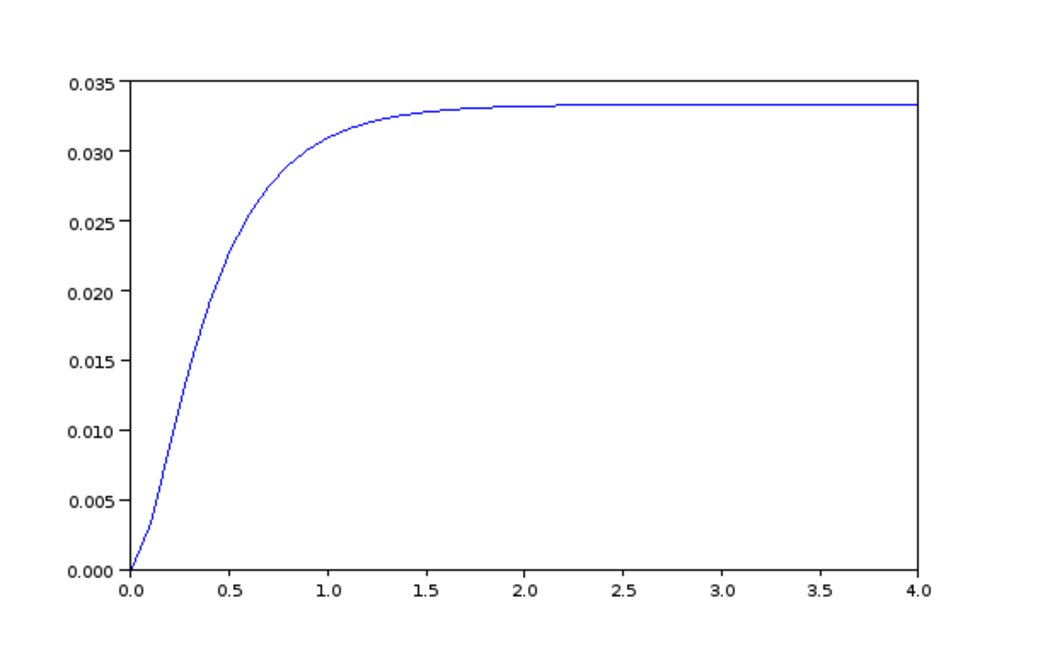
\includegraphics[width=3.0in]{figs05/realstepa.png}
&
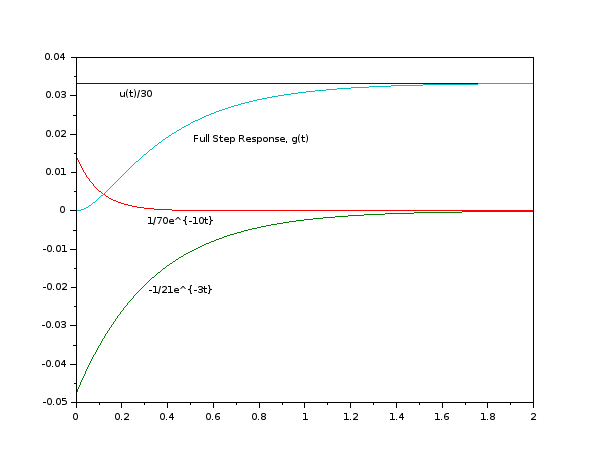
\includegraphics[width=3.0in]{figs05/step_components.png}
\end{tabular}

Note that g(t) has three components,  $0.0333u(t)$, $ - 0.0476 e^{-3t}$, $ +0.0143e^{-10t}$.   Plotting
them separately (Right), we see how they combine to create the response


\end{ExampleSmall}


\begin{ExampleSmall}
Find the poles of the transfer function,
\[
G(s) = \frac{400}{12.7s^2 + 304.8s + 2641.6}
\]
and plot the step response by computer.

\vspace{0.25in}
Applying the quadratic formula to get the roots of the denominator:

\[
\{a,b\} = \frac {-304.8 \pm \sqrt{304.8^2 -4\times12.7\times2641.6}}{2\times 12.7}
\]
\[
\{a,b\} = \{(-12+j8),(-12-j8)\}
\]
In this case the poles are complex numbers.

Note that these numbers were kind of messy. This illustrates a good reason to normalize the denominator polynomial.   Lets do the problem again but with a normalized denominator:

\[
G(s) = \frac{3.15}{s^2 + 24s + 208}
\]
Applying the quadratic formula to get the roots of the denominator:

\[
\{a,b\} = \frac {24 \pm \sqrt{24^2 -4\times208}}{2}
\]
This is simplified because the $s^2$ coefficient (`$a$' in the quadratic formula) is one.  The result is the same.
\[
\{a,b\} = \{(-12+j8),(-12-j8)\}
\]

Plotting the step response by computer:

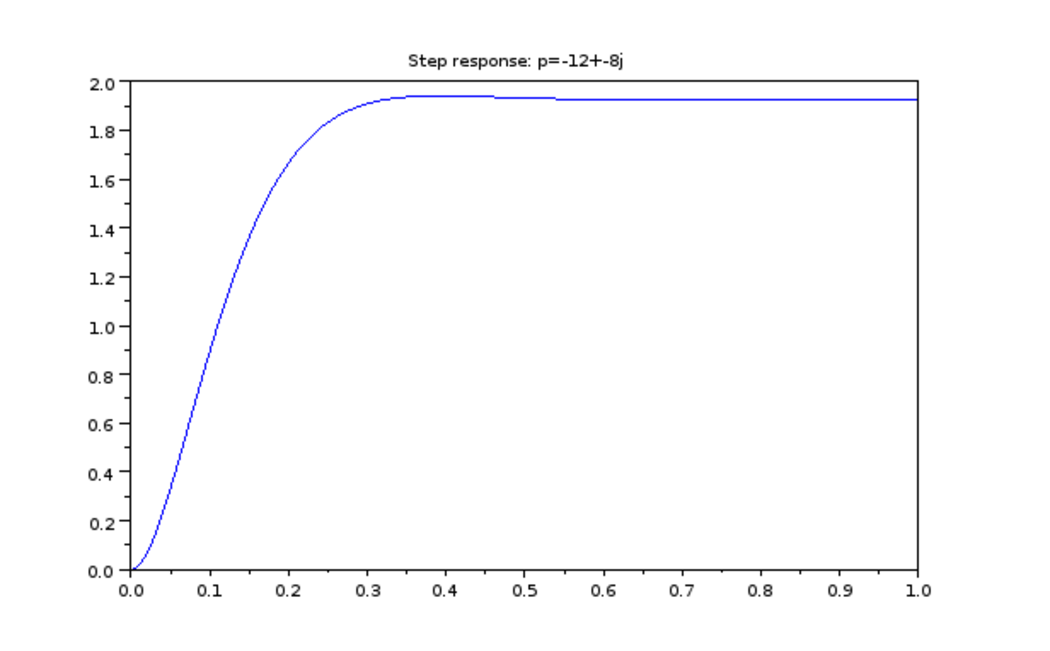
\includegraphics[width=3.5in]{figs05/cplxstepa.png}
\end{ExampleSmall}


There are lots of ways we could express the simple polynomial in the denominator of $G(s)$ and we'll play around with a few:

\[
G(s) = \frac{1}{s^2+us+v} \qquad (u = -(a+b),\quad v= ab)
\]
Now let's introduce a parameter $\omega_n$ (pronounced ``omega-n''):
\[
\omega_n  = \sqrt{v} = \sqrt{ab}
\]
and another one, $\zeta$ (``zeta''):
\[
\zeta = \frac{u}{2\sqrt{v}} = \frac{-(a+b)}{2\sqrt{ab}}
\]

if we make these substitions, our transfer function becomes
\[
G(s) = \frac{1}{s^2 + 2\zeta\omega_n s+\omega_n^2}
\]

So far this is just playing around with notation.  The point  however is that $\zeta$ and $\omega_n$, called the {\it damping ratio} and {\it natural frequency} respectively, give important insights not obvious from the poles ($a,b$) themselves.

If the poles are complex, we know that they must  be complex conjugates of each other. In other words,
\[
Re(a) = Re(b) \qquad Im(a) = -Im(b)
\]

Using the properties of complex numbers, and the fact above, it is simple to show

\[
\omega_n = \sqrt{Re(a)^2 + Im(a)^2} = |a| = |b|
\]
\[
\theta = \tan^{-1}\left(\frac{\omega}{\sigma}\right)= \tan^{-1}\left(\frac{Im(a)}{-Re(a)}\right)
\]
\[
\zeta = \cos(\theta)
\]

If we plot these points on the complex plane (Figure \ref{ccpoleszeta}) we can see why these parameters give a different view from the poles:
they represent the poles in polar coordinates.

\[ \angle a = \cos^{-1}(\zeta), \quad |a| = \omega_n
\]


\begin{figure}\centering
 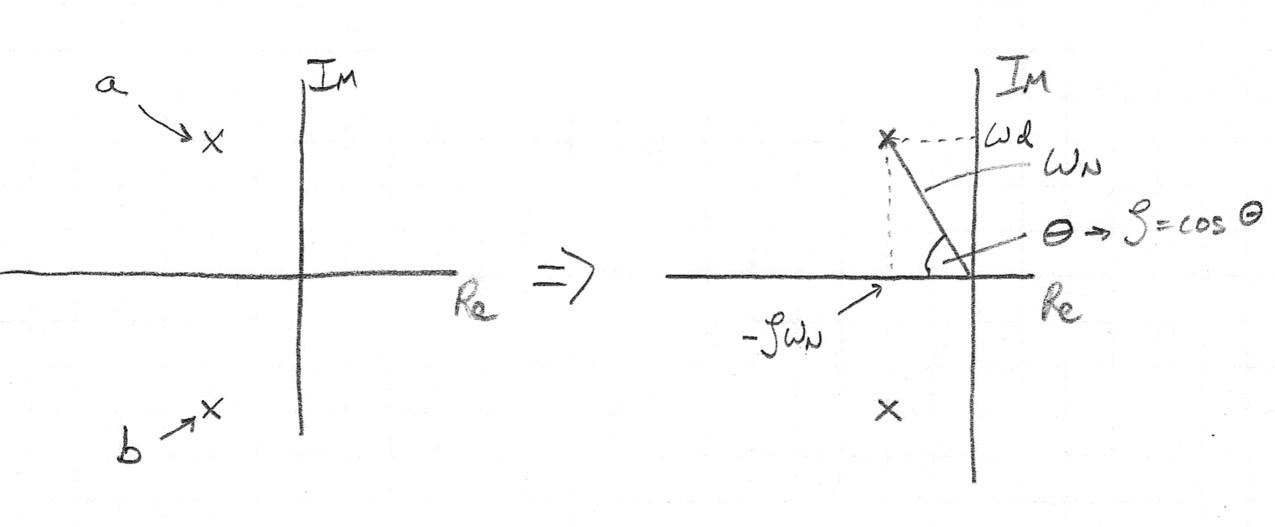
\includegraphics[width=4.25in]{figs05/00733a.png}
\caption{Complex conjugate poles in the complex plane can be represented in Cartesian Coordinates
($\sigma+j\omega$) or polar coordinates $\{\zeta, \omega_n\}$}\label{ccpoleszeta}
\end{figure}

\subsection{Pole Location and Step Response}

The location of poles in the complex plane determines the characteristics of the dynamic response to system inputs.  One input which we care about a lot is the step function

\[
u(t) = \left \{ \begin{array}{cc} 0 & t< 0 \\ 1 & t >= 0 \end{array} \right .
\]

The Laplace transform of the step input is $U(s) = \frac{1}{s}$.

The response to  a step input determines what the system will do when we ``change our minds'' about what the output should be.  For example, you walk into a room and turn the thermostat from $50^\circ$ to $68^\circ$ or you press ``Resume'' on your cruise control.


When we take a 2nd order transfer function of the form $G(s) = \frac{M}{(s+a)(s+b)}$, and multiply it by the step input, we get the output
\[
Y(s) = \frac{1}{s}\frac{M}{(s+a)(s+b)},
\]
we can expand it using the partial fraction expansion (Section \ref{partialfractionsection}) into the form
\[
Y(s) = \frac{A_0}{s} + \frac{A_1}{(s+a)}+  \frac{A_2}{(s+b)},
\]

and further,  the inverse transform of each term in the partial fraction expansion is

\bq\label{dampedexponentialsolution}
y(t) = A_0 +  A_1e^{at} + A_2e^{bt}   \qquad (t>= 0)
\eq

It can be shown (see Example 1.s\ref{Ex:2ndOrderInvTrans}) that for a 2nd order system with a pair of complex conjugate poles, $\{a,b\}$, $A_1=A_2^*$, $|A_1| = |A_2|$, and that this solution takes the form

\bq\label{eqnDampedSinStep}
y(t) = A_0-|A_1|e^{-\zeta\omega_n t} (2\cos({\omega_dt +\phi}))
\eq

In this response, the exponential term {\it multiplies } the sinusoid term.  Since the sinusoid cannot exceed the range $-1<=sin(\omega t)<=1$, the response will be bounded by the exponential and we will call it the ``envelope'' since it ``contains'' the sinusoidal part of the response.
Let's look at some examples of this function.  For $\omega_n = 0.4$, and $\zeta=.124$ (corresponding to the poles: $s = -0.05\pm0.4j$), we get the step response shown in Figure \ref{typicalstep}



\begin{figure}\centering
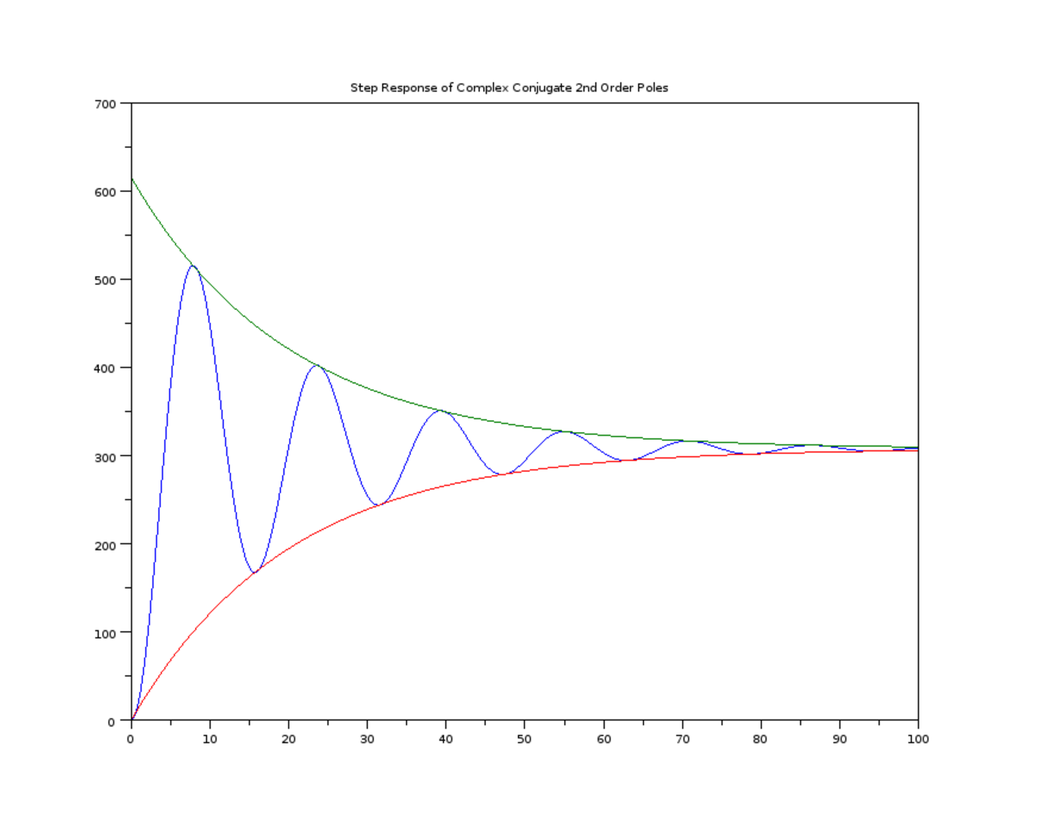
\includegraphics[width=3.5in]{figs05/typical_stepa.png}
\caption{Step response of a typical system ($\omega_n = 0.4, \zeta=.124$ ) with complex conjugate 2nd order poles. The envelopes (red and green) are also shown.}\label{typicalstep}
\end{figure}



Now, let's place these responses according to the location of their complex poles.  Figure \ref{splaneresponse} represents the top half of the complex plane.   Each plot is the response of a 2nd order system having one of its complex conjugate poles in its rough location.  Note that the last two columns have positive real parts to their poles.



\begin{figure}\centering
  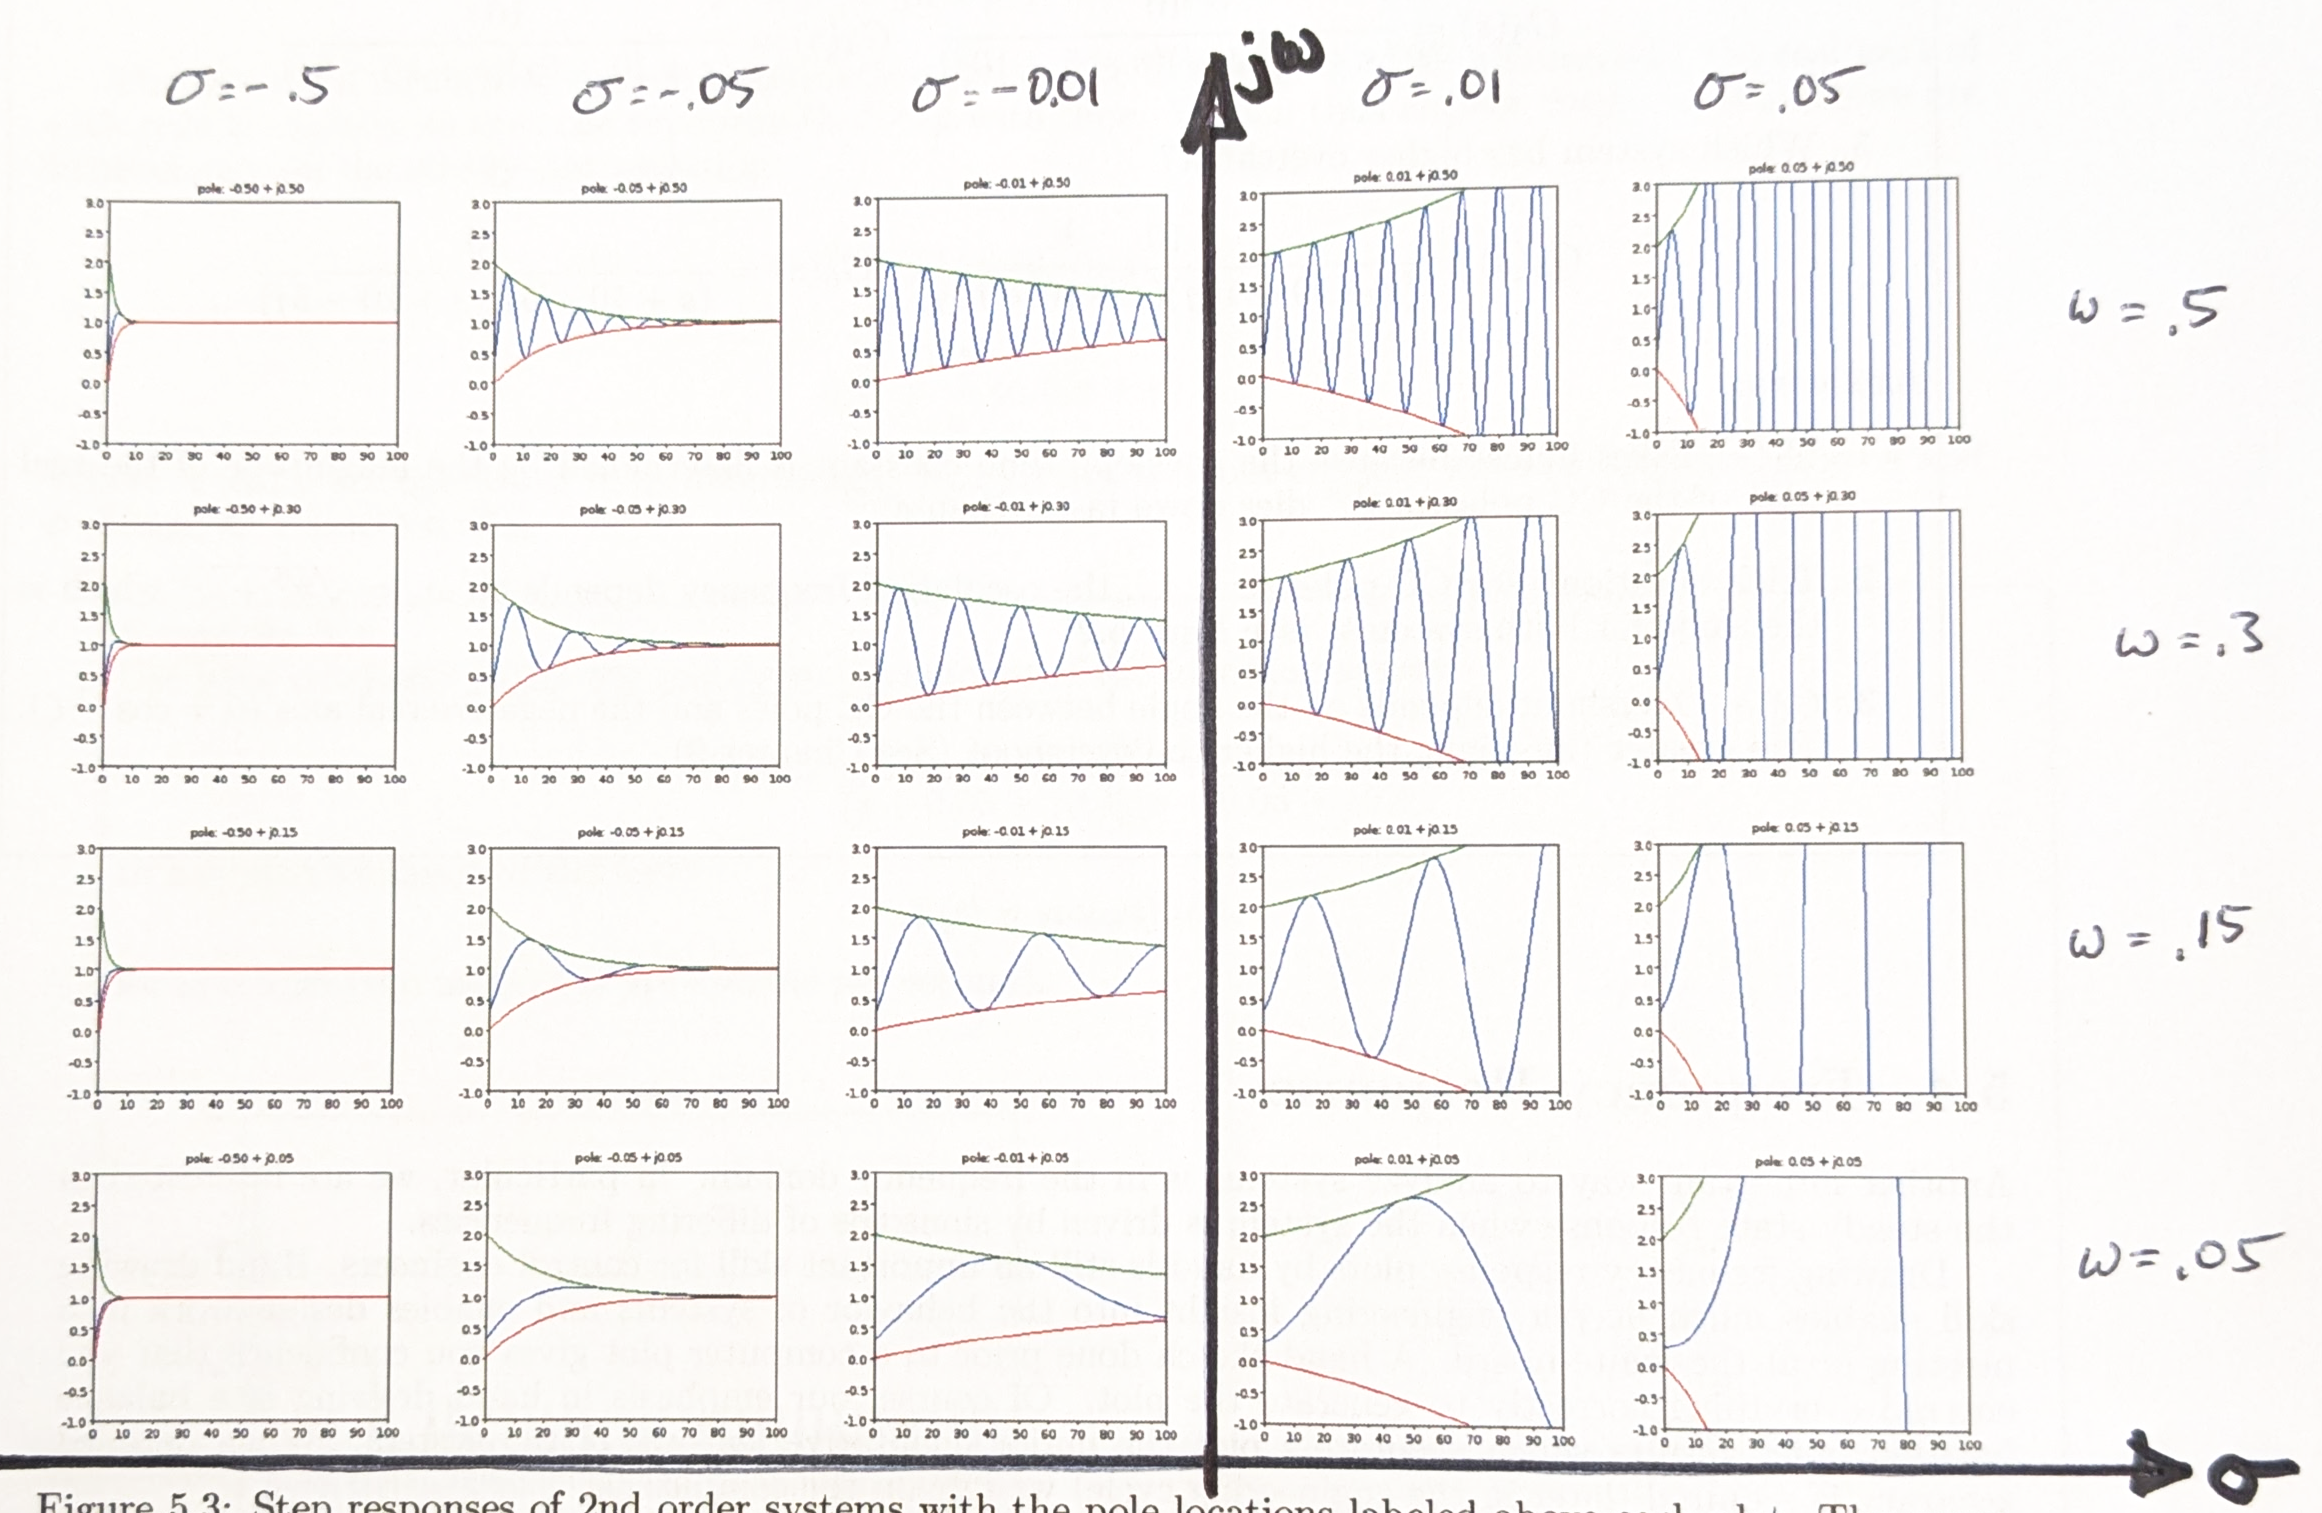
\includegraphics[width=6.5in]{figs05/s_planeResponses_Annotated.png}
  \caption{Step responses of 2nd order systems with the pole locations labeled above each plot. The array of sub-plots represents part of the upper half of the complex plane.}\label{splaneresponse}
\end{figure}


Looking at Figure \ref{splaneresponse} there are two key patterns.  First, the frequency of the sinusoid increases as the imaginary part of the pole increases.  Second the envelope grows with time when the real part is positive, and shrinks over time when the real part is negative.   The larger the magnitude of the real part, the faster the envelope changes.



\begin{Example}
  Test yourself on your knowledge of pole location's effect on step response with these questions:
  \begin{enumerate}
    \item  Which system takes longer for the step response transient to die down?
    \[
    G_1(s) = \frac{10}{(s+5+10j)(s+5-10j)} \quad G_2(s) = \frac{10}{(s+10+5j)(s+10-5j)}
    \]
    \item  Which system has a higher oscillation frequency in the step response transient?
    \[
    G_3(s) = \frac{10}{(s+5+10j)(s+5-10j)} \quad G_4(s) = \frac{10}{(s+10+5j)(s+10-5j)}
    \]

    \item Which system has higher overshoot?
    \[
    G_5(s) = \frac{10}{(s+10+10j)(s+10-10j)} \quad G_6(s) = \frac{10}{(s+10+5j)(s+10-5j)}
    \]
  \end{enumerate}


  \subsubsection*{Answers:}
  \begin{enumerate}
    \item $G_1(s)$  Takes longer because the envelope time constant is determined by the magnitude of
    the real part of the CC poles.   $e^{-10t}$ dies down faster than $e^{-5t}$.

    \item Trick question!   For CC poles: $\sigma \pm j\omega$, the oscillation frequency depends on $\omega_n = \sqrt{\sigma^2+\omega^2}$
    which is the same for both systems! (see Eqn. \ref{eqnDampedSinStep})

    \item $G_5(s)$ Overshoot depends on the angle between the CC poles and the negative real axis ($\theta = \cos^{-1}{\zeta}$).
    The greater the angle, the higher the overshoot (See Chapter 9).
  \end{enumerate}
\end{Example}


\section{Frequency Response}\label{FrequencyResponseSection}

Another important way to analyze systems is in the frequency domain.   In particular, we are interested in the steady state response when the system is driven by  sinusoids of differing frequencies.

Drawing frequency response plots by hand is still an important skill for control engineers.  Hand drawing skill enables much deeper engineering insight into the behavior of systems and enables design work in a meeting or at the white-board.  A hand sketch done prior to a computer plot gives you confidence that you entered everything correctly to generate the plot.  Of course, our emphasis in hand drawing  is   a balance favoring quick results which accurately plot the major qualitative features of the system.  When detailed accuracy is required (later in the engineering cycle) we rely on the computer.

When a system is driven by a sinusoidal input, the output is derived by multiplying the Laplace transform of the sinusoid with the transfer function.  For example:


\[
x(t) = \sin(\omega t)   \Leftrightarrow X(s) = \frac{\omega}{s^2 + \omega^2}
\]
\[
Y(s) =  \frac{\omega}{s^2 + \omega^2} G(s)
\]

The pole corresponding to the sinusoidal input is the root of $s^2+\omega^2$ which is $s=j\omega$.  Since the magnitude of $\sin(\omega t)$ is always 1 (i.e. does not vary with frequency, $\omega$), the key quantity of interest  is the magnitude of the  transfer function, $|G(j\omega)|$(which does vary with frequency).  If the amplitude of the input sinusoid changes from
\[
\sin(\omega t) \to A\sin(\omega t)
\]
The frequency response can simply be scaled by $A$ due to the linearity property.
\[
|Y(j\omega)| = |G(j\omega)| \to |Y(j\omega)| =|AG(j\omega)|=A|G(j\omega)|
\]

Thus we can focus on $|G(j\omega)|$ and get the response for any amplitude or frequency sinusoid.

We can show that the steady state output is also a sinusoid using the partial fraction expansion as we did above with the step response.   Suppose

\[
Y(s) = \frac{\omega}{s^2 + \omega^2} \frac  {M}   {(s+p_1)(s+p_2)(s+p_3)}
\]
Then the partial fraction expansion would be
\[
Y(s) =  \frac{A_0} {s^2+\omega^2} +  \frac{A_1} {(s+p_1)} +  \frac{A_2} {(s+p_2)} +  \frac{A_3} {(s+p_3)}
\]

The last three terms each transform into exponentials like Equation \ref{dampedexponentialsolution}.
We assume that the real part of each pole is negative so that the exponentials decay with time.   We can thus neglect those terms since we are focused only on the steady state solution:


\[
Y(s) =  \frac{A_0} {s^2+\omega^2}
\]

\[
y(t) = \frac{A}{\omega}  \sin(\omega t + \phi)
\]
Where $A$ and $\phi$ are quantities to be determined.   This section is about efficient ways to determine how $A$ and $\phi$ change as a function of $\omega$.


\begin{ExampleSmall}
Use your computer  to get the steady state response of  the following system

\[
G(s) = \frac{50}{(s+0.05+j0.4)(s+0.05-j0.4)}
\]
to a sinusoidal input of the form:
\[
X(t) = \sin(\omega t)u(t)
\]
for $\omega = 1.25$ (the units of $\omega$ are radians per second).


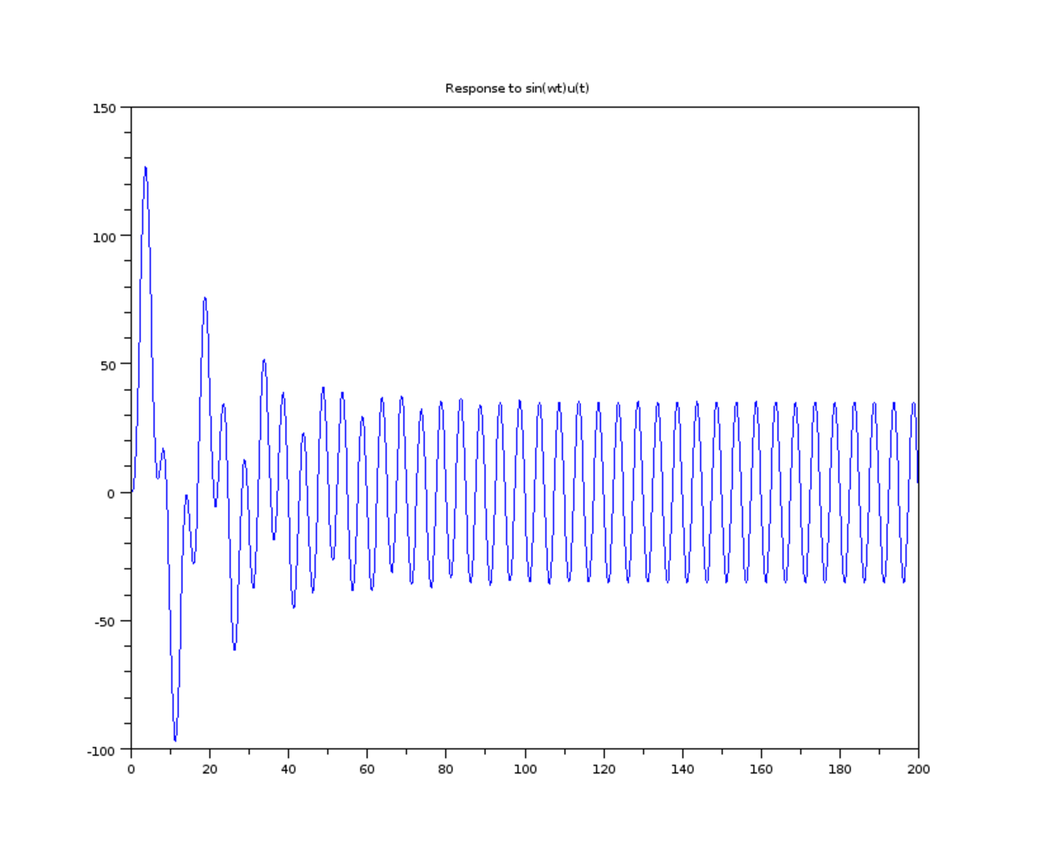
\includegraphics[width=3.5in]{figs05/sinusoid_contina.png}

There is a substantial transient response, but for $t>80$ or so we see the steady state response.

\end{ExampleSmall}





\begin{Example}
  The system
\[
G(s) = \frac{50}{(s+0.05+j0.4)(s+0.05-j0.4)}
\]
is driven by an interrupted  sinusoidal function
\[
x(t) = \sin(1.25t)(u(t)-u(t-100))
\]

Recall that $u(t)$, is the unit step function we learned when studying single sided Laplace Transform analysis with zero initial conditions.  The second term, $-u(t-100)$, when combined with $u(t)$, ``Turns off'' the sinusoid at $t=100$ because for $t>100$, $u(t)-u(t-100) = 0$.
Numerically solving this system on the computer gives a response (below, right) which changes amplitude dramatically at both the turn ON transient ($t=0$) and the turn OFF transient ($t=100$), but settles to a constant sinusoidal output (the {\it steady state} response) for $80< t < 100$.  Note that if the input sinusoid continued forever instead of shutting off at $t=100$, the steady state response would also continue forever.

It is also worth noting that the frequency of the response changes when the input turns off.   This is because the steady state response is a ``forced'' response (i.e. of the same mathematical form as the input), while the turn off transient is a ``natural'' response, i.e. determined by the $\omega_n, \zeta$ of the system.


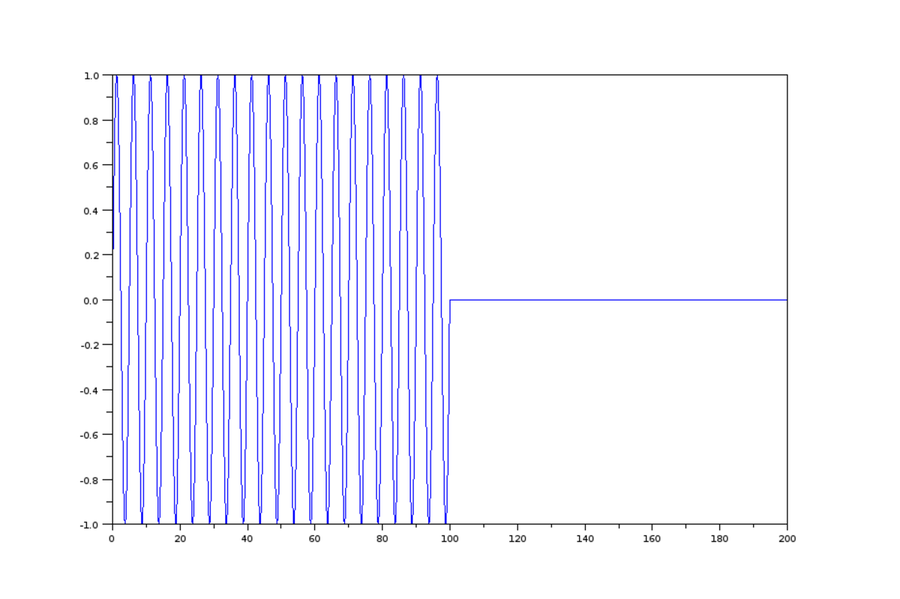
\includegraphics[width=3.in]{figs05/sinusoid_input_stepa.png}
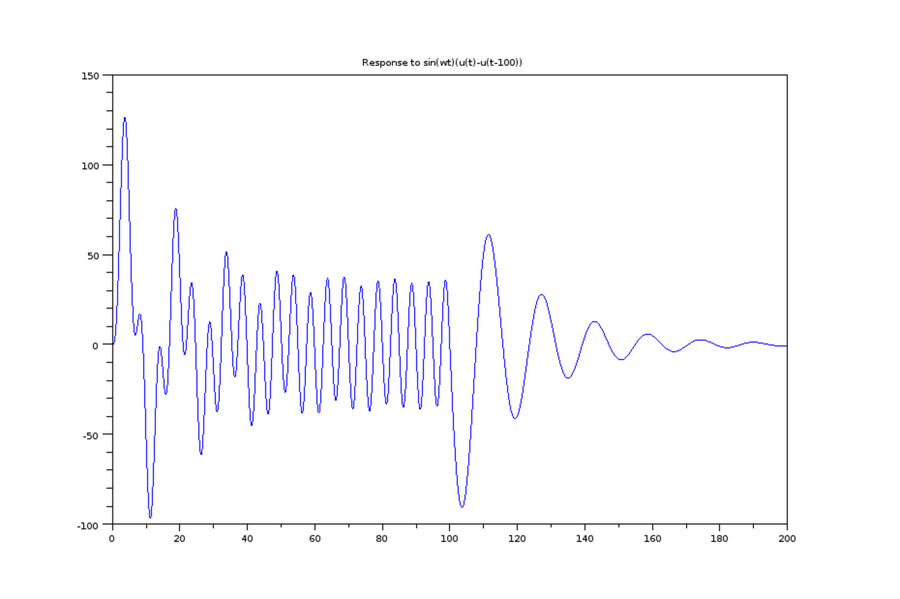
\includegraphics[width=3.in]{figs05/sinusoid_transienta.png}

Left:  Input signal. Right: System response includes transients both when the sinusoid turns ON ($t=0$)and when it turns OFF ($t=100$).
Eventually the ON transient dies out to a steady state response ($75<t<100$).

\end{Example}

Frequency response analysis ignores the transient response (both ON and OFF type) and focuses entirely on the forced, steady state response.  Since the steady state response is always of the same mathematical form as the input, we need only concern ourselves with differences in amplitude and phase (between the input and output sinusoid).



Each root of the denominator of a transfer function is called a pole.  Each root of the numerator is called a zero.  Each pole and zero is a real or complex number which affects how the system
responds to both transient and steady state inputs.

\subsection{Magnitude}

The first task of frequency response analysis of a system described by $G(s)$ is to compute $|G(j\omega)|$ over some frequency range of interest, $\omega_{min} < \omega < \omega_{max}$.
$|G(j\omega)|$ is computed by 1) plugging in $s=j\omega$ and 2) evaluating the magnitude of each pole and zero term, and 3) combining the terms.


\begin{ExampleSmall}\label{examplemagnitude}
Compute the magnitude of
\[
G_1(j\omega) = \frac{10^5(s+12.7)}{(s+0.1)(s+10)(s+5000)}
\]
for $\omega = 100$ rad/sec.  Express the magnitude in $dB$.
\vspace{0.25in}

Plugging in
\[
|G_1(j100)| = \frac {10^5(12.7 + j100)}     {(0.1+j100)(10+j100)(5000+j100)}
\]
Evaluating the magnitude of each term:
\[
|G_1(j100)| = \frac {10^5(\sqrt{12.7^2 + 100^2})}     {(\sqrt{0.1^2+100^2})(\sqrt{10^2+100^2})(\sqrt{5000^2+100^2})}
\]

\[
|G_1(j100)| = \frac {10^5(100.8)}     {(100.000005)(100.5)(5001)}
\]
Combining

\[
|G_1(j100)| = 0.20056
\]

Some observations about this computation follow:


\begin{enumerate}
  \item  The computations have been carried out to excessive precision.   Practical control plants are rarely known to even 1\% accuracy.
  \item  Another reason for excessive precision above is that we did not neglect any terms.   In practice, a term like $|0.1+j100|$ can be instantly replaced with $100$ since we know the $0.1^2$ is going to be insignificant.  (Don't do this when the real and imaginary parts are close in magnitude!)
  \item  In an application where highly accurate numerical values must be obtained, we can use computer software.
 In modern engineering, hand calculations (even with a calculator) should only aim at quick approximate results.
\end{enumerate}

\end{ExampleSmall}


\subsection{Phase}

Phase shift between the input and the output is represented by the angle of the complex transfer function evaluated at frequency $\omega$.   Phase is computed by a similar procedure to magnitude:
1) plugging in $s=j\omega$ and
2) evaluating the phase of each pole and zero term, and
3) combining the terms.




\begin{ExampleSmall}\label{examplephase}
Compute the phase angle of
\[
G_1(j\omega) = \frac{10^5(s+12.7)}{(s+0.1)(s+10)(s+5000)}
\]
for $\omega = 100$ rad/sec.  Express the angle  in degrees.
\vspace{0.25in}

Plugging in
\[
\angle G_1(j100) = \angle \frac {10^5(12.7 + j100)}     {(0.1+j100)(10+j100)(5000+j100)}
\]
Evaluating the angle of each term and subtracting denominator angle from numerator angle:
\[
\angle G_1(j100) = \left( {\tan^{-1}({0/10^5})+(\tan^{-1}(100/12.7)}\right) - \left(     {(\tan^{-1}(100/0.1))+(\tan^{-1}(100/10))+(\tan^{-1}(100/5000))} \right)
\]

\[
\angle G_1(j100) = 0^\circ + 82.76^\circ  -   89.94^\circ - 84.30^\circ - 1.146^\circ  = -92.626^\circ
\]

The observations of Example \thechapter.\ref{examplemagnitude} apply almost exactly to the phase computation as well.

\end{ExampleSmall}






\subsection{Decibels}

Decibels are a logarithmic\footnote{Take the quiz and review logs if necessary: Section \ref{LogReview}} unit which are widely used for the analysis of frequency response.   If we have a quantity, $x$, then
\[
dB(x) = 20\log_{10}(x)
\]
where $dB(x)$ represents the decibel representation of $x$.


Because decibels are logarithmic units, we will make frequent use of the following properties (which are easily proved using basic properties of logarithms)

\[
dB(ab) = dB(a)+ dB(b)
\]
\[
dB(a/b) = dB(a) - dB(b)
\]
\[
dB(\sqrt{a}) = \frac {dB(a)}{2}
\]
etc.

Some handy {\it approximate} $dB$ values, when  memorized, give you very quick and accurate (within 5\%) hand calculation results:

\[
3.16 = \sqrt{10} = 10dB ,\quad 10 = 20dB, \quad 100 = 40dB
\]
\[
2 = 6dB, \quad   \sqrt{2} = 3dB
\]
\[
1/2 = -6dB, \quad \frac{1}{\sqrt{2}} = \frac{\sqrt{2}}{2} = -3dB
\]
etc.


\begin{ExampleSmall}
Convert the following quantities to $dB$.

\[
dB(1000) = 20\log(1000) = 20*3 = 60dB
\]
\[
dB(6000) = dB(1000\times6) = dB(1000) + dB(6)  = 60 + 15.6 = 76.6dB
\]
\[
dB(X/100) \quad (\mathrm{where }\quad dB(X)=40dB) = 40 - 20\log(100) = 40-40 = 0dB
\]

\end{ExampleSmall}


\begin{ExampleSmall}\label{quickmagwithdb}
Taking into account the points raised in Example \thechapter.\ref{examplemagnitude}, Let's redo the magnitude computation and get a quick approximate answer:


Plugging in
\[
|G_1(j100)| = \frac {10^5(12.7 + j100)}     {(0.1+j100)(10+j100)(5000+j100)}
\]
Quickly evaluating the magnitude of each term by neglecting the small parts :
\[
|G_1(j100)| \approx \frac {10^5(100)}     {(100)(100)(5000)}
\]
Converting to $dB$


\[
|G_1(j100)| = 100dB + 40dB - 2*40dB - 60dB - 20\log(5) = -14dB
\]


\end{ExampleSmall}


\begin{ExampleSmall}
Convert the magnitude calculation of Example \thechapter.\ref{examplemagnitude} to $dB$ and compare it with Exercise \thechapter.\ref{quickmagwithdb}.


Converting to $dB$:
\[
dB(2.0056) = -14dB
\]
which is the same result.
\end{ExampleSmall}

\subsection{Bode Plot Sketching}\label{BodePlotAsymptoticApprox}

The Bode asymptotic magnitude plot (named after famous Bell Labs engineer Hendrik Bode, 1905-1982)
is a log-log plot of magnitude vs. freqency, and is usually used with the Bode asymptotic phase plot which is a linear-linear plot of phase vs. frequency.  Bode's key contribution was to understand that the key properties of $|G(j\omega)|$ and $\angle G(j\omega)$ can be obtained by sketching straight line asympotes which are easily identified from the transfer function.   In the 1930s, this replaced hours of tedious hand calculation.   Today, we get an accurate Bode plot from the computer in seconds, but the asymptotic hand sketch has two key remaining insights:


\begin{enumerate}
  \item  We can quickly estimate frequency response on the back of an envelope or at the white-board during group work.
  \item  We gain key insights about which parameters of the transfer function are responsible for which features of the frequency response.
\end{enumerate}


\subsubsection{Bode Asymptotic Magnitude Plot (BAMP)}


\paragraph{Single Pole}

We start by looking at a simple transfer function consisting of one pole:

\[
G(s) = \frac{1}{(s+a)}\quad (\mathrm{here, our pole is }\; p=-a)
\]

In all frequency response analysis we assume that $Re(p) < 0$.  For now we assume $Im(p) = 0$.

We consider $s=j\omega$ and there are three values of $\omega$ which are relevant.

\begin{enumerate}
  \item  $\omega << |p|$
  \item  $\omega = |p|$
  \item  $\omega >> |p|$
\end{enumerate}

Ranges 1 and 3 are ``asympotic'' because they become more and more true as $|\omega| \to 0$ or $|\omega| \to \infty$. Value 2 is an exact value  so we can easily compute an ``anchor point'' for the graph.
For each region, as we plug in $s=j\omega$, we can approximate $|G(j\omega)|$ as

\begin{enumerate}
  \item  $|G(j\omega)| = \left | \frac{1}{j\omega+a} \right |  \approx 1/a$
  \item  $|G(j\omega)| = \left | \frac{1}{a+ja}    \right |       =    \frac {1} {\sqrt{a^2+a^2}} = \frac{1}{a}\frac{1}{\sqrt{2}}$
  \item  $|G(j\omega)| = \left | \frac{1}{j\omega+a} \right |  \approx \left | \frac{1}{j\omega} \right | = \frac{1}{\omega}$
\end{enumerate}

Importantly, the Bode Magnitude plot is logarithmic in the Magnitude and we express Magnitude in $dB$.
Therefore we can re-write the  approximations  as

\begin{enumerate}
  \item  $|G(j\omega)| \approx -dB(a)$
  \item  $|G(j\omega)| = \left | dB(\frac{1}{a+ja})    \right | = dB(\frac{1}{\sqrt{a^2+a^2}) =
    dB(a^-1}+dB(\frac{1}{\sqrt{2}}_ = -dB(a) - dB(\sqrt{2}) = -dB(a) -3dB$
  \item  $|G(j\omega)| \approx \left | dB(\frac{1}{j\omega}) \right | = -dB(\omega)$
\end{enumerate}

If we plot this on a log-log scale, we get Figure \ref{BodeMagOnePole}.
It's important to note a couple of things.

\begin{enumerate}
  \item The low frequency asymptote is horizontal because it is constant with respect to $\omega$, ($-dB(a)$).
  \item The high frequency asymptote ( $-dB(\omega)$) intersects
         the low frequency asymptote ( $-dB(a)$) at $\omega = a, |G(ja)| = -dB(a)$.
  \item The actual curve is smooth and intersects the point
  $\{\omega=\log(a), |G| = -dB(a)-3dB\}$ in accordance with
  the calculation for  $\omega = a$.

  \item As $\omega$ gets greater than $a$, the magnitude drops with frequency according to
  $$ M = -dB(\omega) $$

In log-log coordinates, $-dB(\omega)$ is a straight line with a slope of -1.  When we say ``slope of -1'', we mean the magnitude drops a factor of 10 for every factor of 10 increase in $\omega$.   We express this slope as $\frac{-20dB}{\mathrm{decade}}$. The term ``decade'' refers to an order of magnitude change of frequency.

\end{enumerate}


\begin{figure}\centering
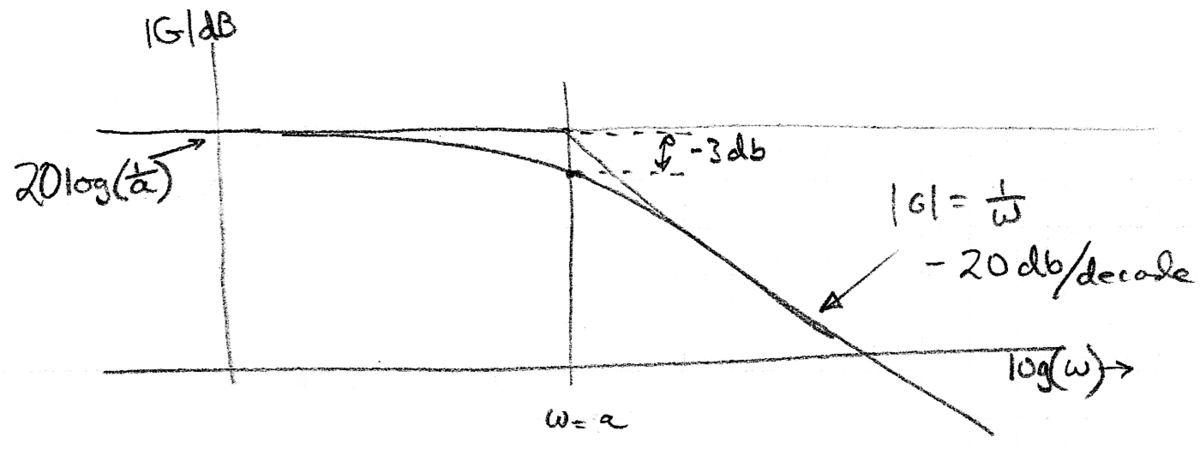
\includegraphics[width=4.0in]{figs05/00734a.png}
\caption{Bode Magnitude Plot of a single pole.}\label{BodeMagOnePole}
\end{figure}


\paragraph{Single Zero}
Now we consider the case of a system represented by

\[
G(s) = \frac{(s+a)}{1}
\]

As before, we assume $Re(p) < 0$.  For now we assume $Im(p) = 0$.

The same three ranges of $\omega$ are relevant:

\begin{enumerate}
  \item  $\omega << |a|$
  \item  $\omega = |a|$
  \item  $\omega >> |a|$
\end{enumerate}

For each region, as we plug in $s=j\omega$, we can approximate $|G(j\omega)|$ as

\begin{enumerate}
  \item  $|G(j\omega)| \approx a$
  \item  $|G(j\omega)| \approx \left | a+ja \right | = a\sqrt{2}$
  \item  $|G(j\omega)| \approx \left | j\omega \right | = \omega$
\end{enumerate}

Again, the Bode Magnitude plot is logarithmic in the Magnitude and we express Magnitude in $dB$.
Therefore we can re-write the  approximations  as

\begin{enumerate}
  \item  $|G(j\omega)| \approx dB(a)$
  \item  $|G(j\omega)| \approx \left | dB(\frac{1}{a+ja})    \right | = dB(a)+3dB$
  \item  $|G(j\omega)| \approx \left | dB(\frac{1}{j\omega}) \right | = dB(\omega)$
\end{enumerate}

If we plot this we get Figure \ref{BodeMagOneZero}.

The zero plot is identical to the pole plot except inverted (reflected around the line $|G| = 0dB$).
The slope of the high-frequency asymptote is now +1 or $+20dB/\mathrm{decade}$.


\begin{figure}\centering
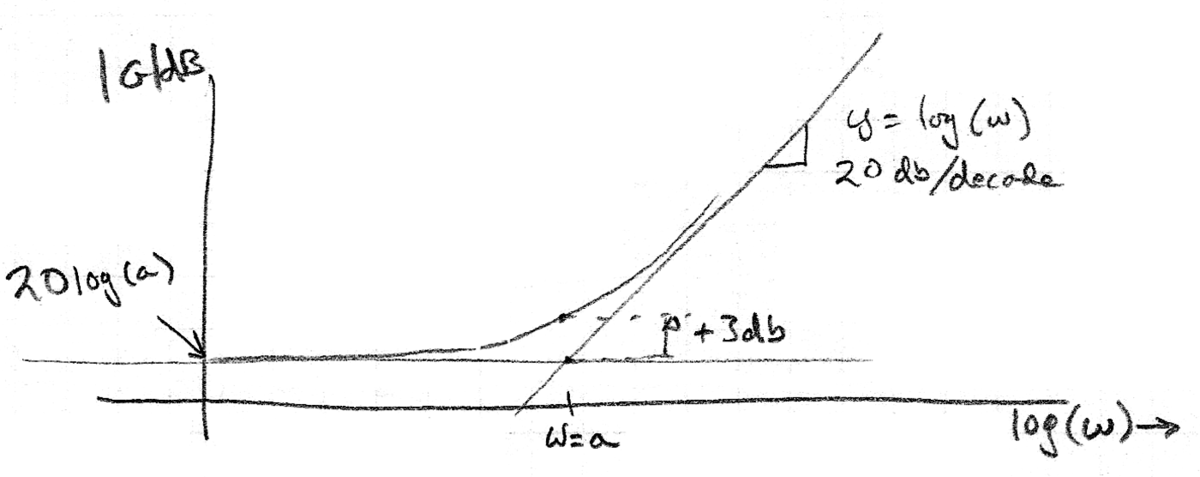
\includegraphics[width=4.0in]{figs05/00735a.png}
\caption{Bode Magnitude Plot of a single zero.}\label{BodeMagOneZero}
\end{figure}


Note that these graphs are generic for any value of $a$.   If they are multiplied by any different amplitude, $A$, then they can be decomposed as follows:

\[
|G_A(s) | = \left | \frac {A} {(s+a)} \right | =  |A|  \left | \frac {1} {(s+a)} \right | = dB(A) + dB \left ( \left | \frac {1} {(s+a)} \right | \right)
\]

In other words they are shifted up or down by $dB(A)$.




\begin{ExampleSmall}
Plot the Bode Asymptotic Magnitude Plot for the following single-pole transfer function:
\[
G_2(s) = \frac  {2000} {(s + 200.0)}
\]

As above we can decompose this into
\[
\mathrm{dB}(|G_2(s)|)  = dB(2000) - dB(|(s+200)|)
\]

Thus the Bode plot of Figure \ref{BodeMagOnePole} directly applies as long as we add $dB(2000) = 66dB$ and we have


\begin{enumerate}
  \item The intersection of the two asymptotes is at $\omega=200$.
  \item The low frequency (horizontal) asymptote is at
  \[
   |G_2(j\omega)| = 66dB + (-46dB) = 20dB
  \]
  Where $66dB$ comes from the factor of 2000, and $-46dB$ comes from $20\log(1/200)$.    Drawing the asymptotes and drawing the smooth curve through $20dB - 3dB$ at $\omega=\log(200)$.

  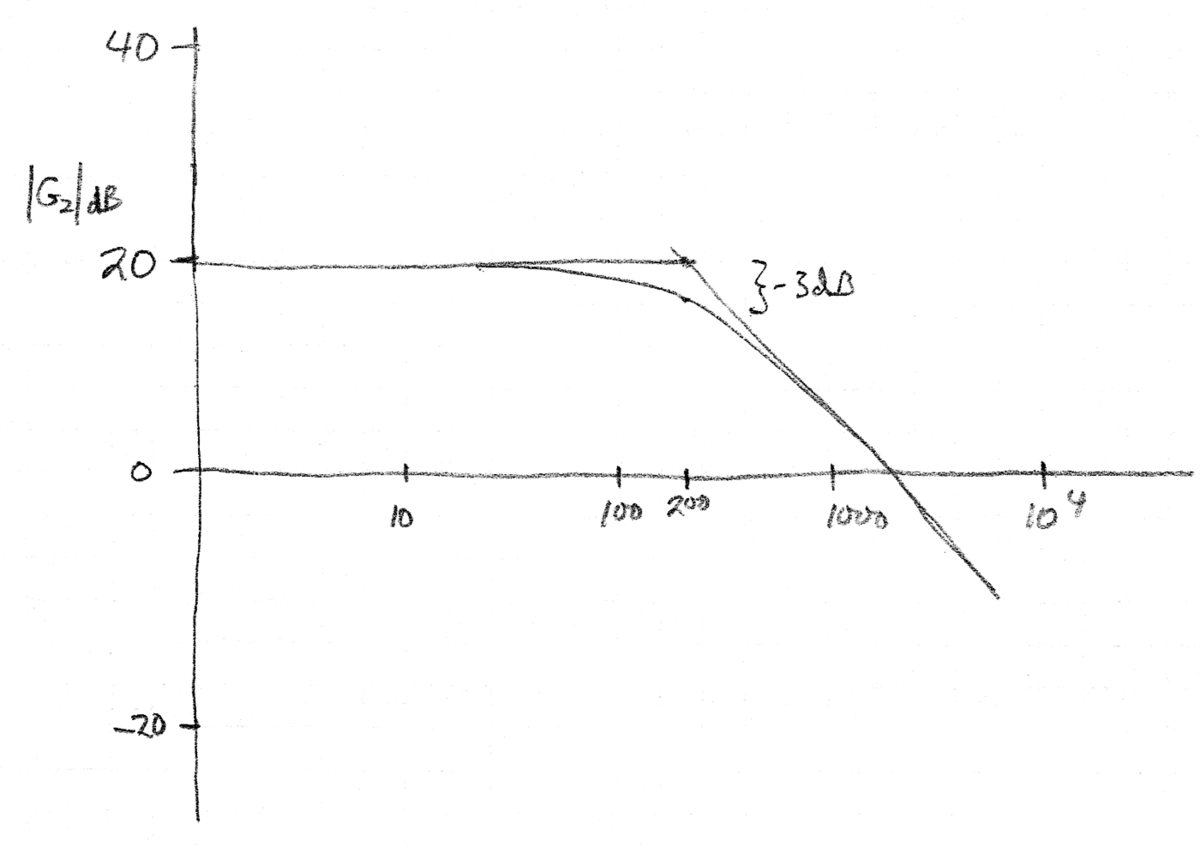
\includegraphics[width=4.0in]{figs05/00736a.png}
\end{enumerate}




\end{ExampleSmall}



\subsection{Combining Magnitude Plots}

Consider the more realistic transfer function which has one zero and two poles:

\[
G_3(s) = \frac    {(s+b)} {(s+a)(s+c)}
\]

We will define the {\it features} of the transfer function to be the  poles and zeros.
In $G_3$ for example,
\[
\frac {1} {(s+a)} \qquad {(s+b)} \qquad\frac {1} {(s+c)}
\]
which we may just call $a,b,c$ for short, are all {\it features} of $G_3(s)$.

To make a Bode Asymptotic Magnitude plot of this more interesting function, we recognize that it is the product of two poles and one zero:

\[
G_d(s) = \frac {1} {(s+b)}  \frac {(s+a)} {1}  \frac {1} {(s+c)}
\]
and since we are plotting in a $dB$ scale that
\[
dB(|G_3(s)|) =  dB(\left |\frac {1} {(s+b)}\right |) +   dB(\left |\frac {(s+a)} {1}\right | ) +  dB( \left | \frac {1} {(s+c)}\right |  )
\]
In other words, we can just add the three Bode plots together.   This is a valid way to do it but is still time consuming because four total plots have to be made.   To find a simpler way, let's constrain the first asympotic frequency range slightly so that it is below the lowest feature, i.e.

\[
\omega <<  \mathrm{min}(a,b,c)
\]

For this case
\[
|G_3(\omega)| = dB(a) - dB(b)  - dB(c)
\]
at this point we know where the low frequency (horizontal) asymptote intersects the $dB$ axis.
Assume that in $G_3(s)$ the smallest feature is $a$.
An important way to look at the basic plots of Figures \ref{BodeMagOnePole} and \ref{BodeMagOneZero} is that they are horizontal for $\omega < $ the lowest feature, and sloped (either down for poles or up for zeros) for $\omega > $ the lowest feature.
Thus, the quickest way to draw the Bode Asymptotic Magnitude plot is to start from the horizontal asymptote and then,
as log frequency increases, to add in a component of slope as $\omega$ gets to each pole or zero.


\subsection{``Cartoon'' Bode Magnitude Plot}\label{CartoonBode}
It is useful at this stage to make a cartoonish version of the Bode Magnitude plot using only
our knowledge of the order of the features (from low to high frequency). This can be done in
seconds.  Suppose
\[
G_4(s) = \frac  {(s+1)}  {(s+50)(s+1000)}
\]
in frequency order we have:
\begin{enumerate}
  \item A zero at $s=1$
  \item A pole at $s=50$
  \item A pole at $s=1000$
\end{enumerate}

Without worrying about precise locations in the log-log plane, we can immediately
draw:

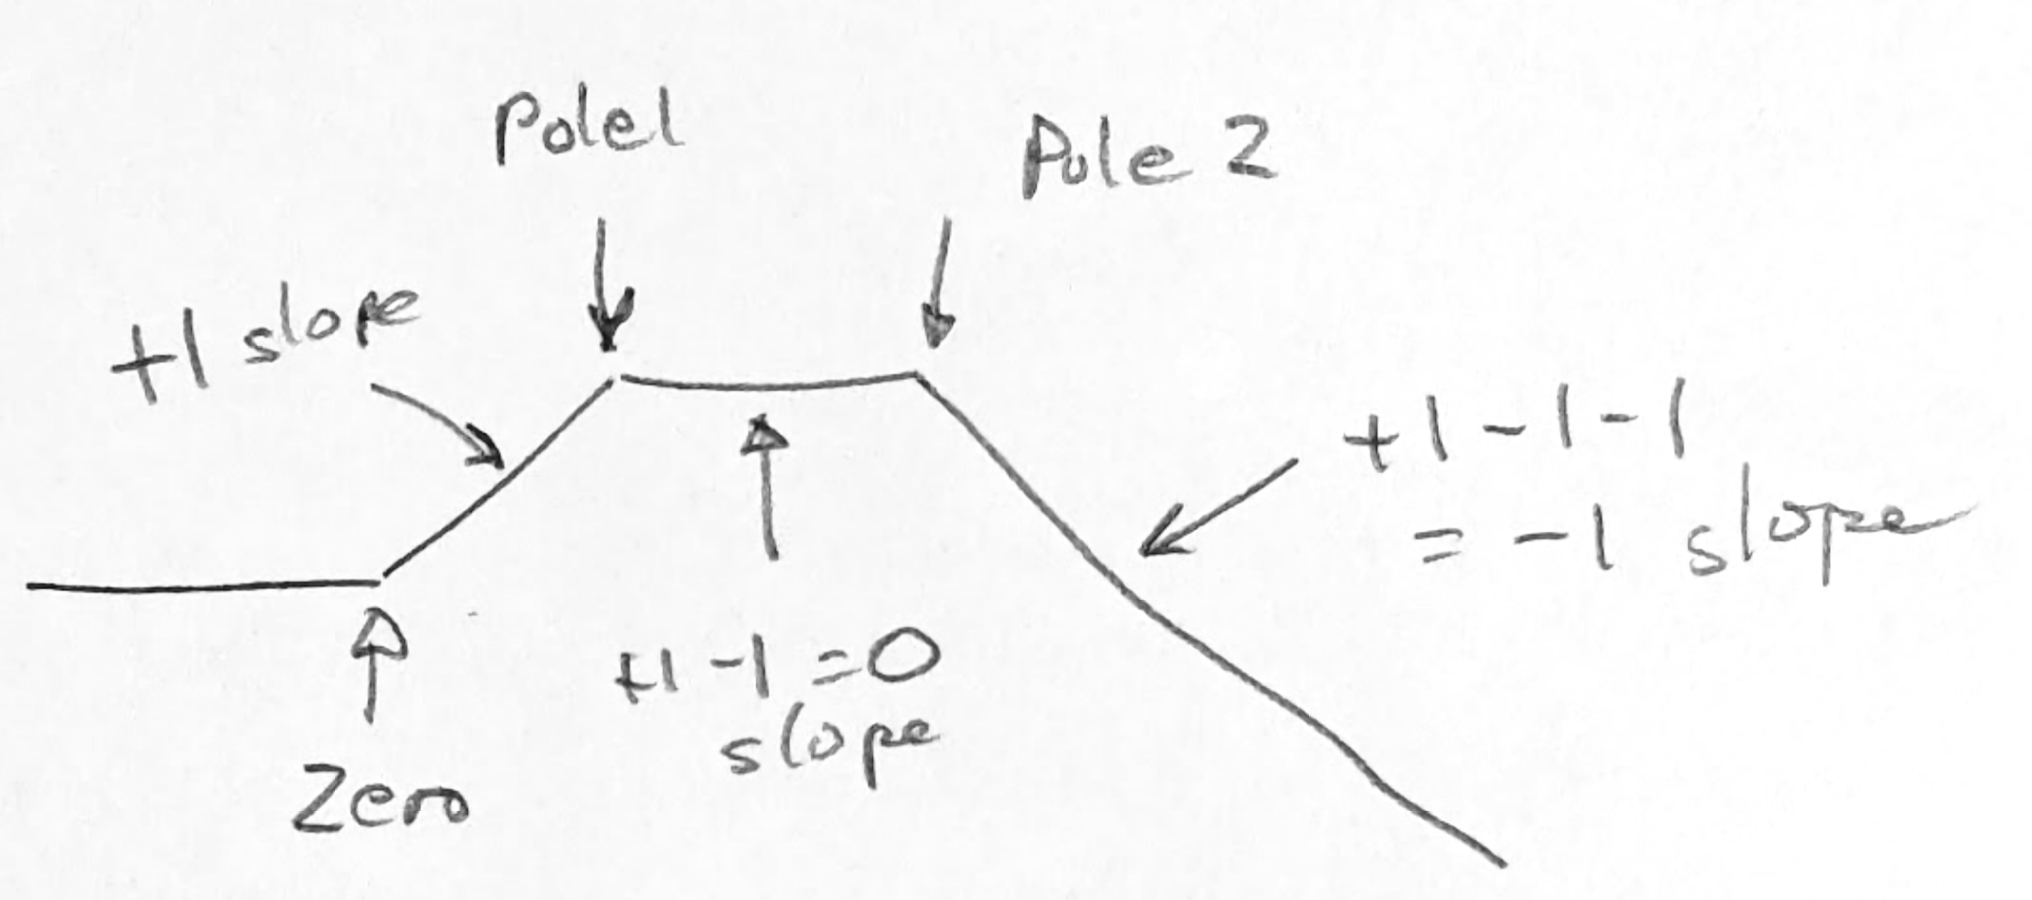
\includegraphics[width=80mm]{figs05/Q47M85.png}

This works because we are always adding the basic pole zero responses together (multiplication
 in a log axis) which have either
+1 or -1 slope {\it after} their pole/zero frequency but not before.
This gives us the basic idea of how the graph will look.

The quick cartoon Bode plot is useful for example, to
determine what range of $dB$s to use on our y axis and what frequencies to use on our x axis.

\begin{Example}
Draw the ``Cartoon'' Bode magnitude plot for each of the following three transfer functions:

\begin{center}
\[
C1(s) = \frac {(s+10)}  {(s+200)(s+3000+j5000)(s+30000-j5000)}
\]
(draw the slopes in order from the lowest to highest feature, adding or subtracting as you go)

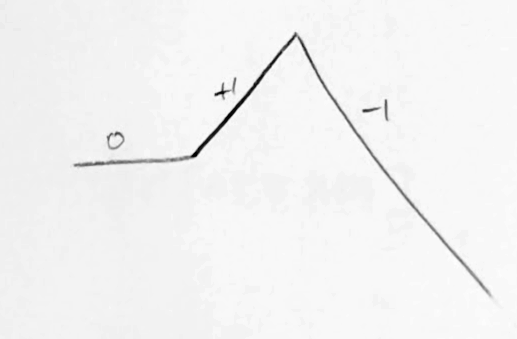
\includegraphics[width=0.3\textwidth]{figs05/J14R56.png}


\[
C2(s) = \frac {(s+1000)^2}  {(s+100)(s+500)}
\]
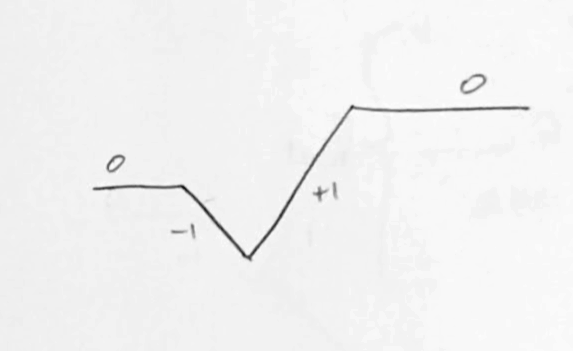
\includegraphics[width=0.3\textwidth]{figs05/J14R57.png}


\[
C3(s) = \frac {(s+2)}  {s(s+500)}
\]
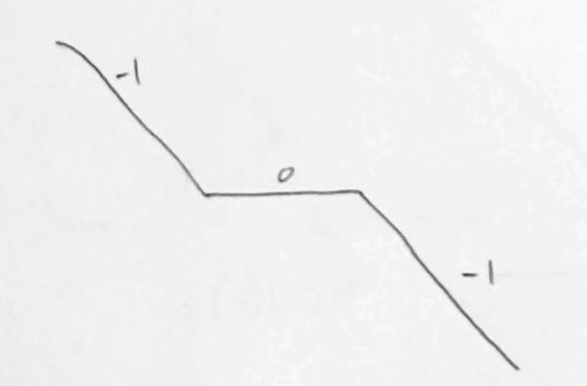
\includegraphics[width=0.3\textwidth]{figs05/J14R58.png}
\end{center}


\end{Example}



\begin{Example}\label{firstBodeMagexample}
Hand draw the Bode Asymptotic Magnitude Plot for

\[
G_4(s) = \frac  {(s+0.1)}  {(s+2)(s+25)}
\]
for the frequency range 0.01 --- 1000 rad/sec.  The order of poles and zeros here
is the same as described above so the cartoon version is the same as that of Section \ref{CartoonBode}.

{\bf Follow these steps:}

1) Find a flat part of the cartoon where it is easy to compute magnitude.   $s=0$ is the
easiest place to compute magnitude and our cartoon is flat for low frequencies.
Compute the magnitude for $\omega << \min(0.1, 2, 25)$ i.e. $\omega << 0.1$.
\[
|G_4(s)| = dB(0.1) - dB(2) - dB(25) = -20dB - 6dB - 28dB = -54dB
\]

2) Draw your log-log axes.

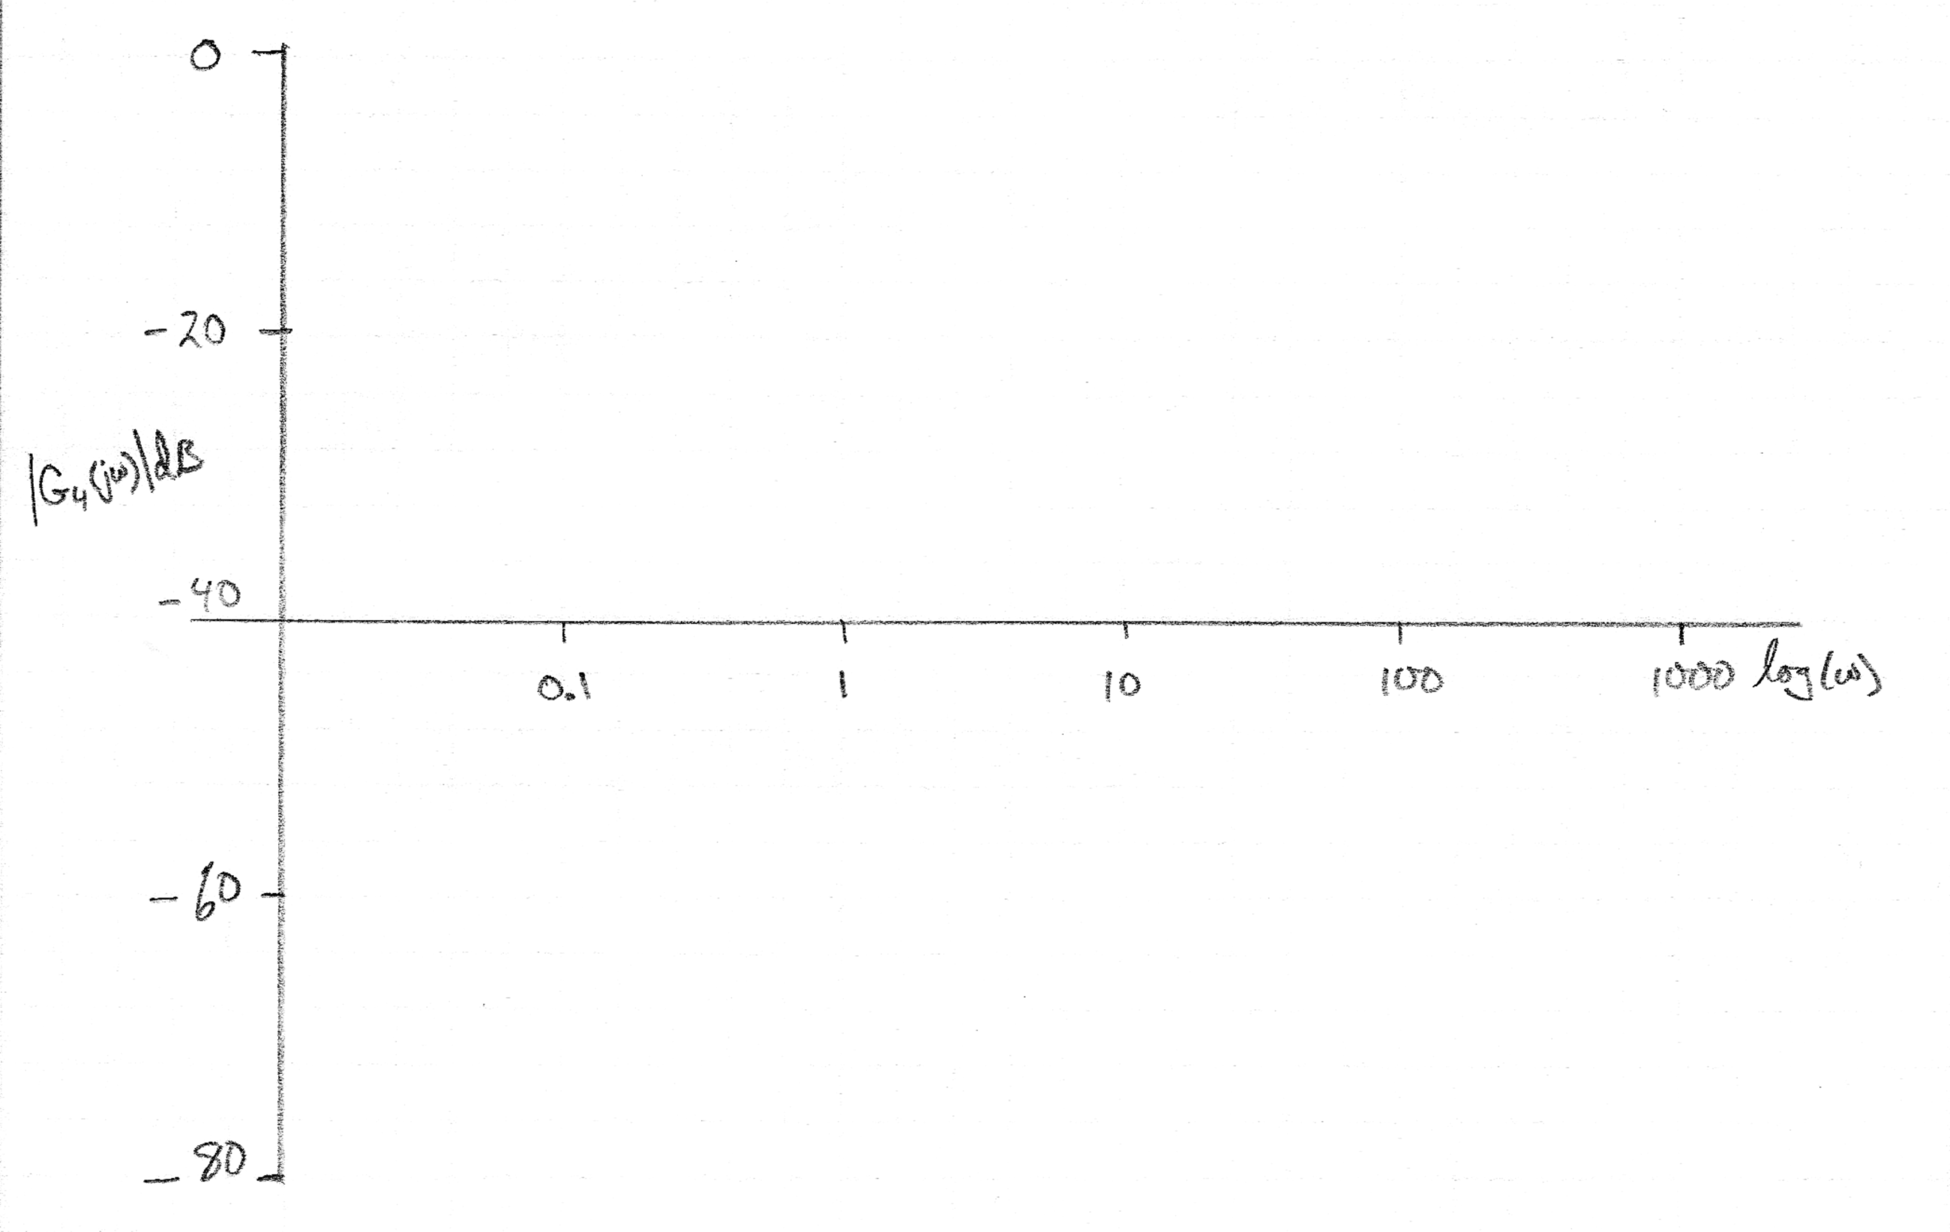
\includegraphics[width=6.5in]{figs05/00737a.png}

Notes about the axes:
\begin{itemize}
  \item It is {\it important } to make the scale (size of a factor of 10)
  the same on both horizontal and vertical axes.
  Verify that this property holds for the above axes (keeping in mind that $20dB = 20\log(10)$).

  \item Although they are given here, use your cartoon and the methods below
  to choose the ranges of $dB$ and $\omega$ to plot.

  For $\omega$ start with $\omega_{min} = 0.1 \min(p_i, z_i)$ (where $p_i$ and $z_i$ are your poles and zeros) and $\omega_{max} = 10 \max(p_i,z_i)$.

  For $dB$ range, your cartoon tells you if your plot will slope upward (zeros first) or downward (zeros at higher frequencies than poles).  Then place your magnitude value obtained in step one near the bottom or top of the range respectively.
\end{itemize}


\end{Example}



\begin{ExampleCont}
\noindent
Continuing our steps:

3) Mark the zero and pole frequencies on the $\log(\omega)$ scale.   Don't forget to take the log of $\omega$ before you mark it down.

4) Starting from the left, draw the low frequency horizontal asymptote (at $-54dB$) to the left up through our first feature, $\omega = 0.1$.  At that frequency, the slope changes to +1 (+20dB/dec) due to the zero so draw an asymptote intersecting the horizontal at $\omega=0.1$ and extending up at $+45^\circ$.

Next at $\omega=2$, we encouter the second feature, the pole at $\omega=2.0$. This pole contributes a negative slope and thus cancels the positive slope.  Draw a new horizontal asymptote (slope =0) intersecting the upward line at $\omega=2$.   Finally, at $\omega = 25$, we have two negative slopes due to the two poles and still the one positive slope from the zero back at $\omega = 0.1$.  The net result is -1 slope for frequencies above 25.

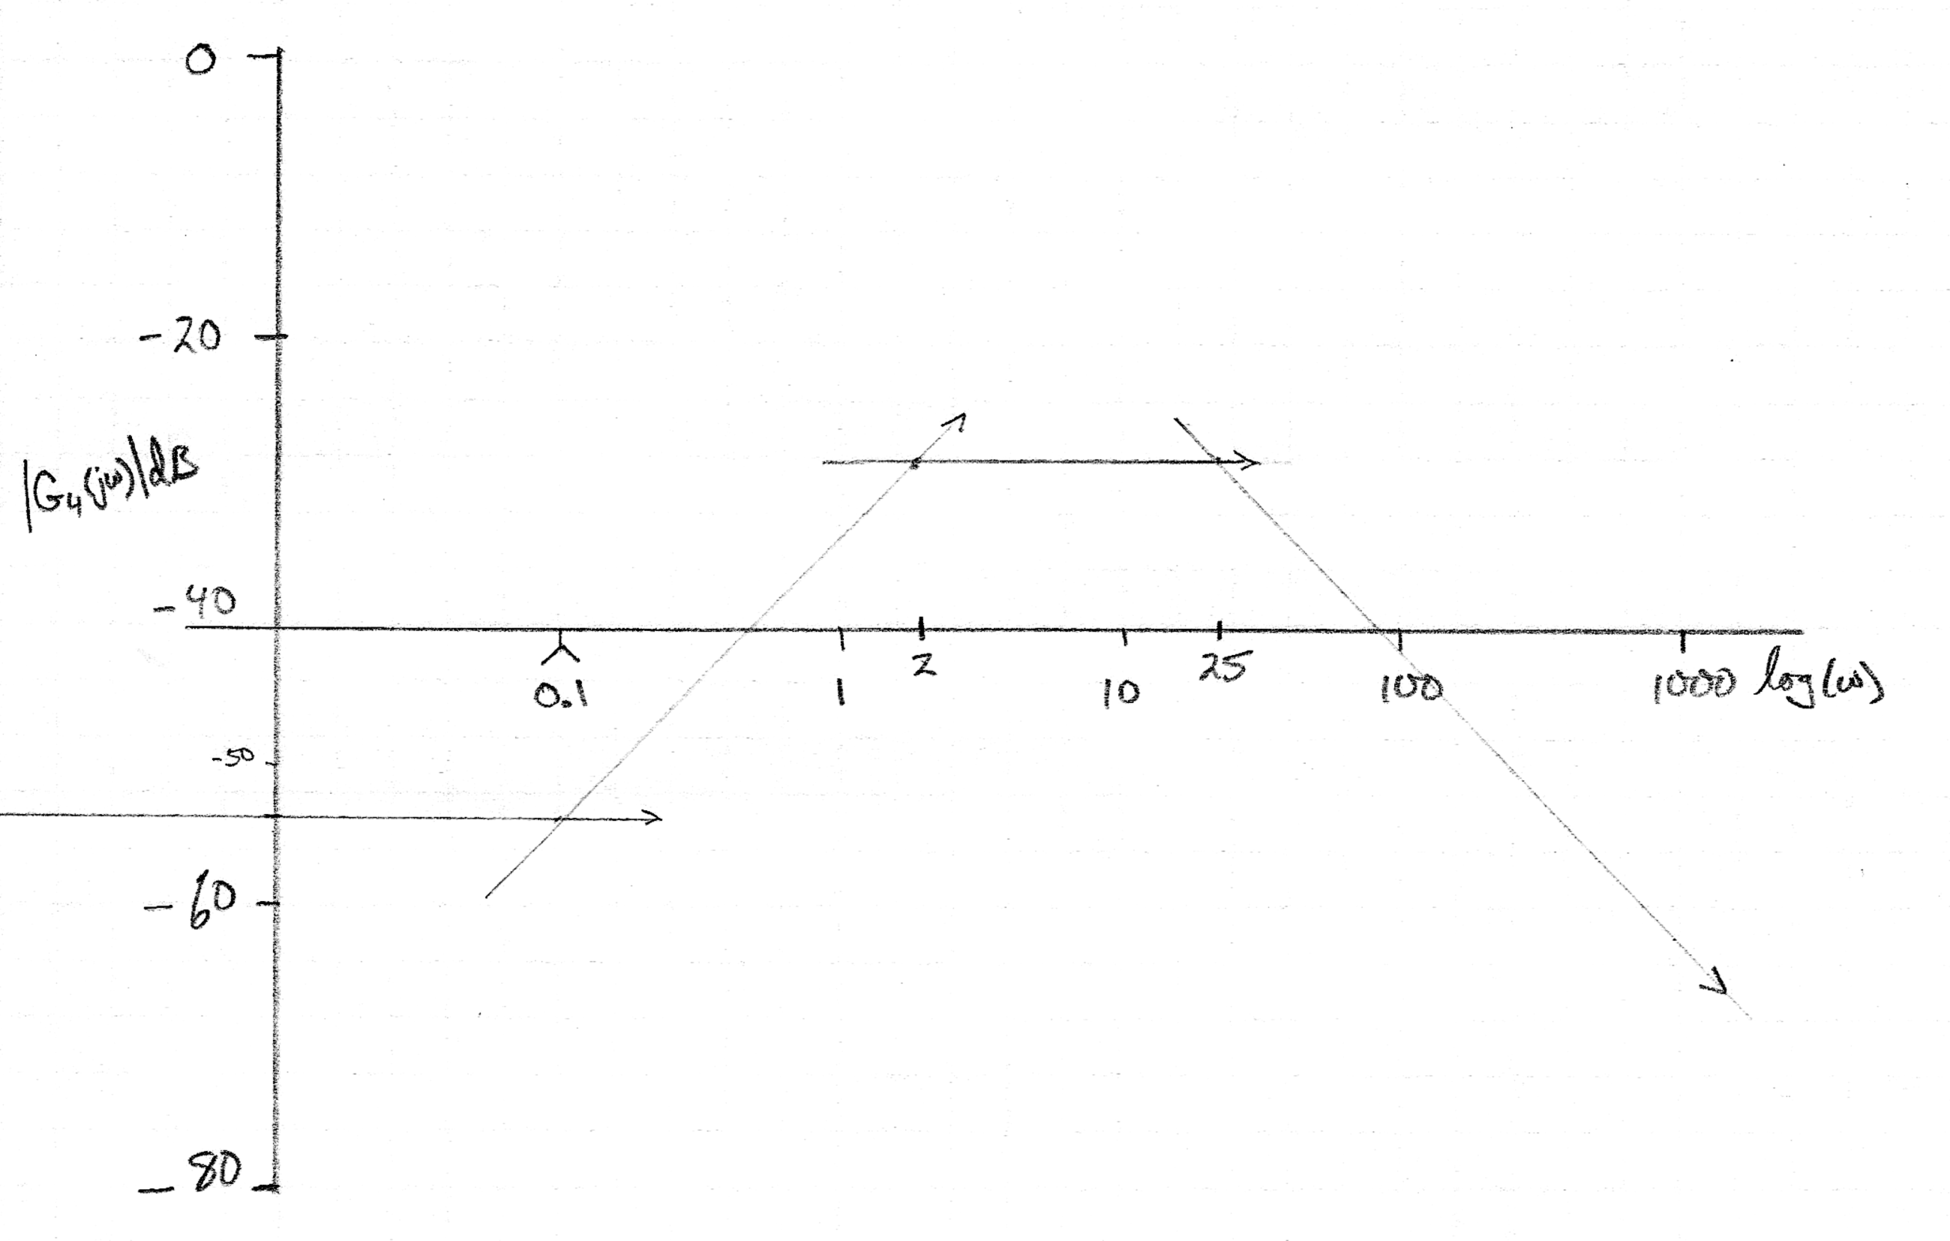
\includegraphics[width=6.5in]{figs05/00738a.png}

5) Mark corrections:   $-3dB$ at each pole ( $\omega = p_i$),   $+3dB$ at  each zero ($\omega=z_i$)

6) Draw a smooth curve through each $3dB$ point.  For a pole, start at $p_i/10$, draw a smooth curve through the $-3dB$ correction, and merge smoothly back into the asymptote at $10p_i$.   Some artistic skill helps here.  When poles or zeros are closer than a factor of 10 apart, you have to blend the smooth curves.  See the range $2.0 < \omega < 25$ in the final plot below.
\end{ExampleCont}


\begin{ExampleCont}
The final plot looks like:

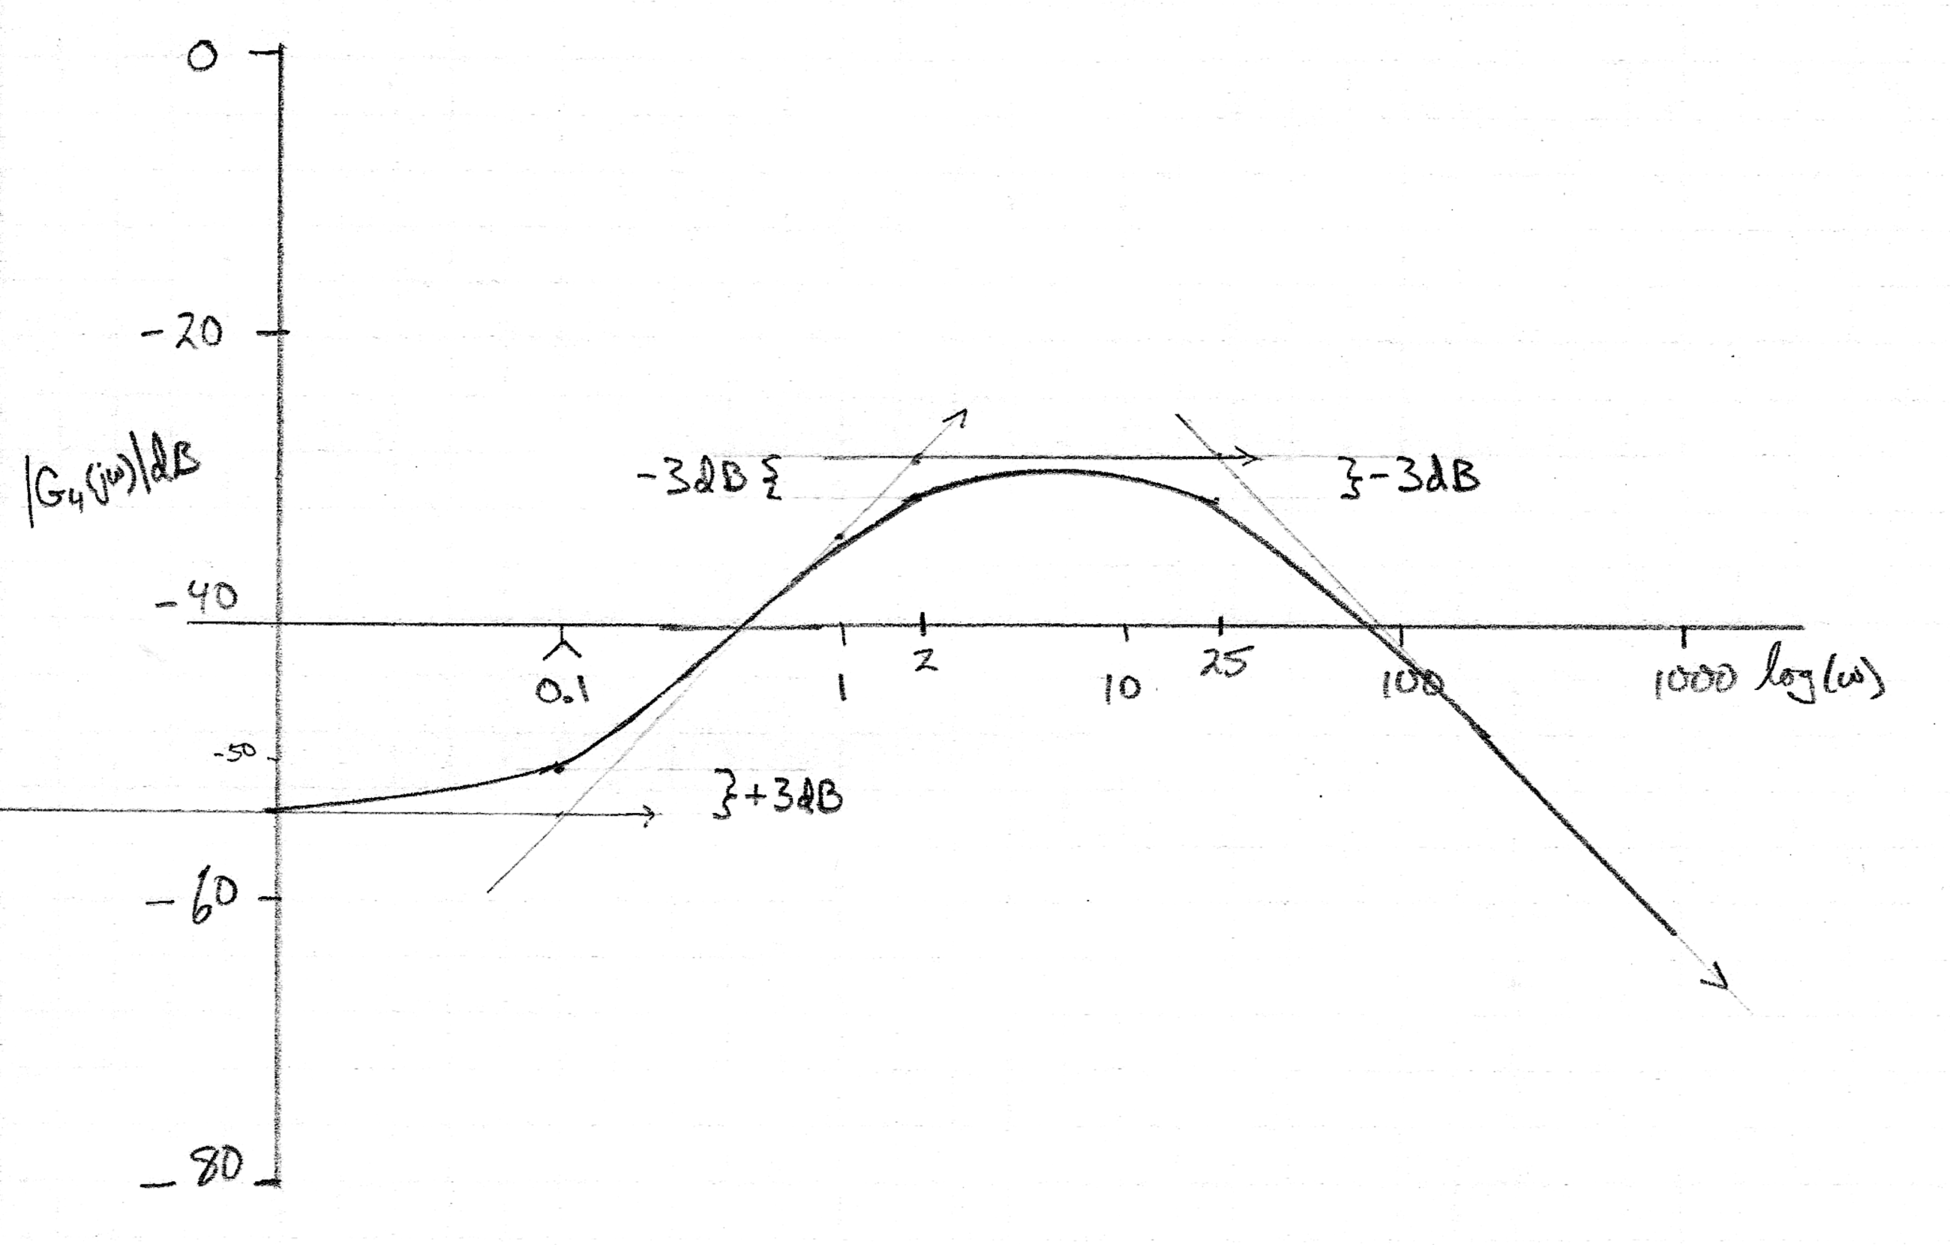
\includegraphics[width=6.5in]{figs05/00739a.png}


{\bf Important Note: }  We did not have to explicitly work out the approximations of Section \ref{BodePlotAsymptoticApprox},
and we did not add three Bode plots together.


\end{ExampleCont}




\subsection{Bode Asymptotic Phase Plot}

We will derive the Bode Asymptotic Phase Plot the same way as the magnitude: by considering three values of $\omega$ relative to the pole or zero.

\paragraph{Single Pole}

Again, we start by looking at a simple transfer function consisting of one pole:

\[
G(s) = \frac{1}{(s+a)}
\]

In all frequency response analysis we assume that $Re(p) < 0$.  For now we assume $Im(p) = 0$.
We consider $s=j\omega$ and there are three values of $\omega$ which are relevant.
The Bode phase  plot uses a linear vertical axis for the phase angle (but uses the same $\log(\omega)$ horizontal axis).

\begin{enumerate}
  \item  $\omega << |a|$
  \item  $\omega = |a|$
  \item  $\omega >> |a|$
\end{enumerate}

For each region of the three regions,
as we plug  $s=j\omega$ into $ \frac{1}{(s+a)}$, we   approximate $|G(j\omega)|$ as

\begin{enumerate}
  \item  $\angle G(j\omega)   \approx 0$
  \item  $\angle G(j\omega) = \angle \frac{1}{a+ja}   =  -45^\circ $
  \item  $\angle G(j\omega) \approx \angle  \frac{1}{j\omega}  = -90^\circ$
\end{enumerate}


If we plot this we get Figure \ref{BodePhaseOnePole}. The figure shows three increasingly accurate approximations to the true phase curve.  Based on the asymptotic approximations above, we get asymptotes which look like a step function which changes from $0^\circ$ to $-90^\circ$ as $\omega$ increases past $a$.
A better approximation is a linear relationship passing through the points
\[
\{\omega=0.1a, \phi = 0^\circ\}, \{\omega=a, \phi = -45^\circ\}, \{\omega=10a, \phi=-90^\circ\}
\]
Finally, by making a smooth curve first above, and then below the linear approximation we can get quite close to a numerically accurate phase curve.  In manual plotting, the intent is not high numerical accuracy, just quick insight.   For precise phase curves, the computer is better.

\begin{figure}\centering
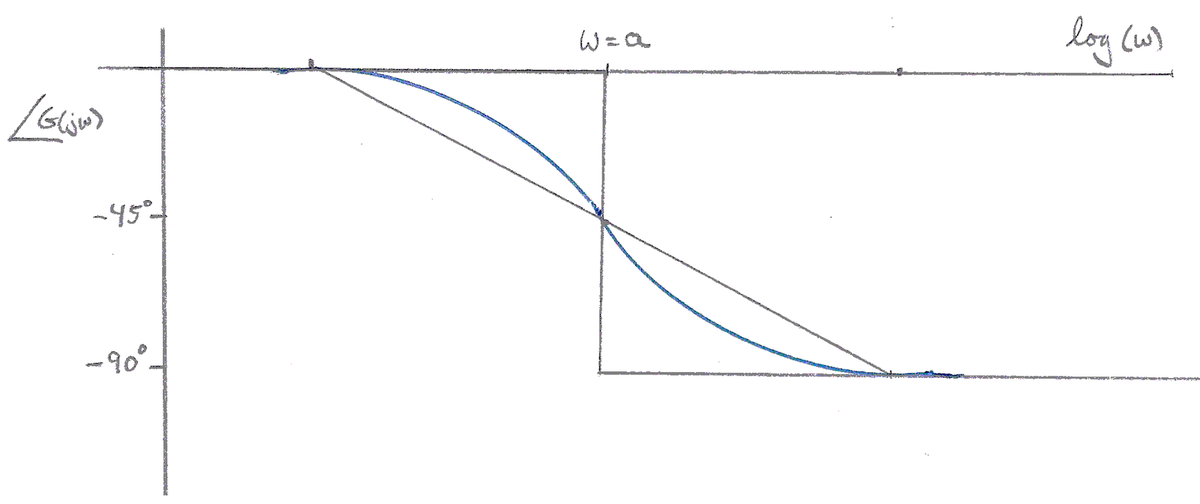
\includegraphics[width=4.0in]{figs05/00757a.png}
\caption{Bode Phase Plot of a single pole. Three approximations of increasing accuracy are given.  1) Straight line (step) asymptotes.  2) linear approximation between $0.1a < \omega < 10a$, 3) Smooth curve passing through $-45^\circ$ at $\omega=a$.}\label{BodePhaseOnePole}
\end{figure}

\paragraph{Single Zero}
By very similar arguments, you can show that a zero such as

\[
G(s) = (s+a)
\]

Contributes the same type of phase curve except flipped above the $0^\circ$ horizontal axis.

\paragraph{Combining Phase Curves}

Just as we can add the Bode Asymptotic Magnitude plots of several poles and zeros (due to the log() nature of $dB$), we can add asymptotic phase curves from the different poles and zeros of a transfer function because the angles of two complex numbers add together when you multiply them.

\begin{Example}

Draw the Bode Asymptotic Phase Plot for the system of Example \thechapter \ref{firstBodeMagexample},
$G_4(s) = \frac  {(s+0.1)}  {(s+2)(s+25)}$

For $\omega < 0.1$ the two poles and  zero each contributes $0^\circ$.  The zero will begin first and contribute $+90^\circ$, then, as $\omega$ increases, the  poles will each contribute $-90^\circ$.   Starting from the left at $\phi=0^\circ$, and drawing only the ``step function'' asymptotes,


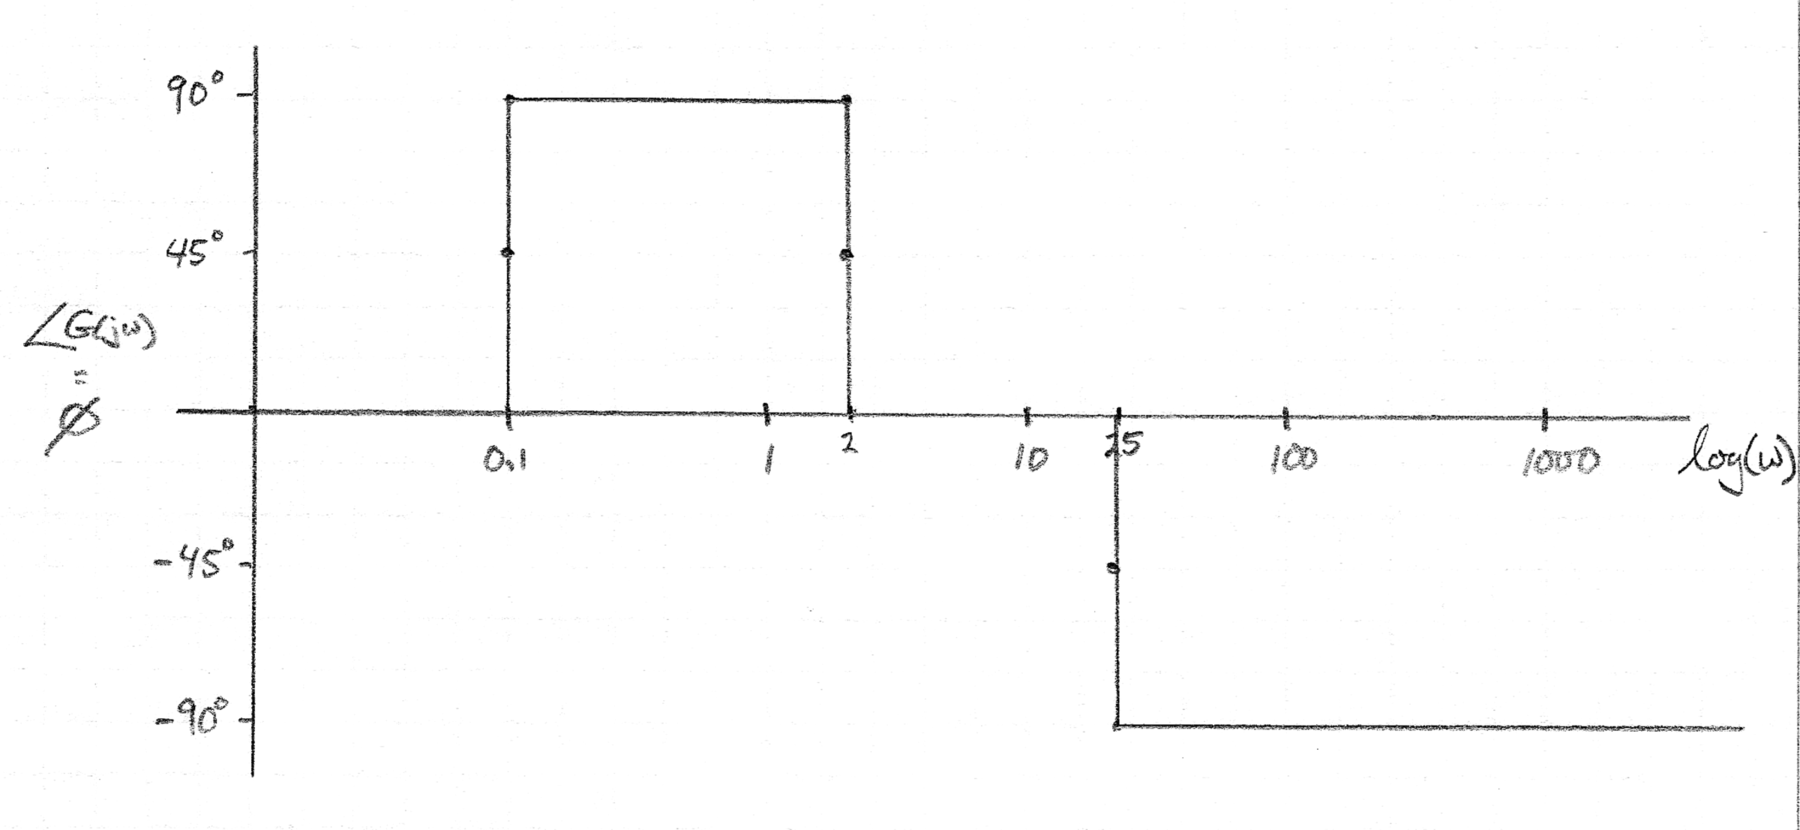
\includegraphics[width=5.5in]{figs05/00758a.png}

Adding in the linear approximations

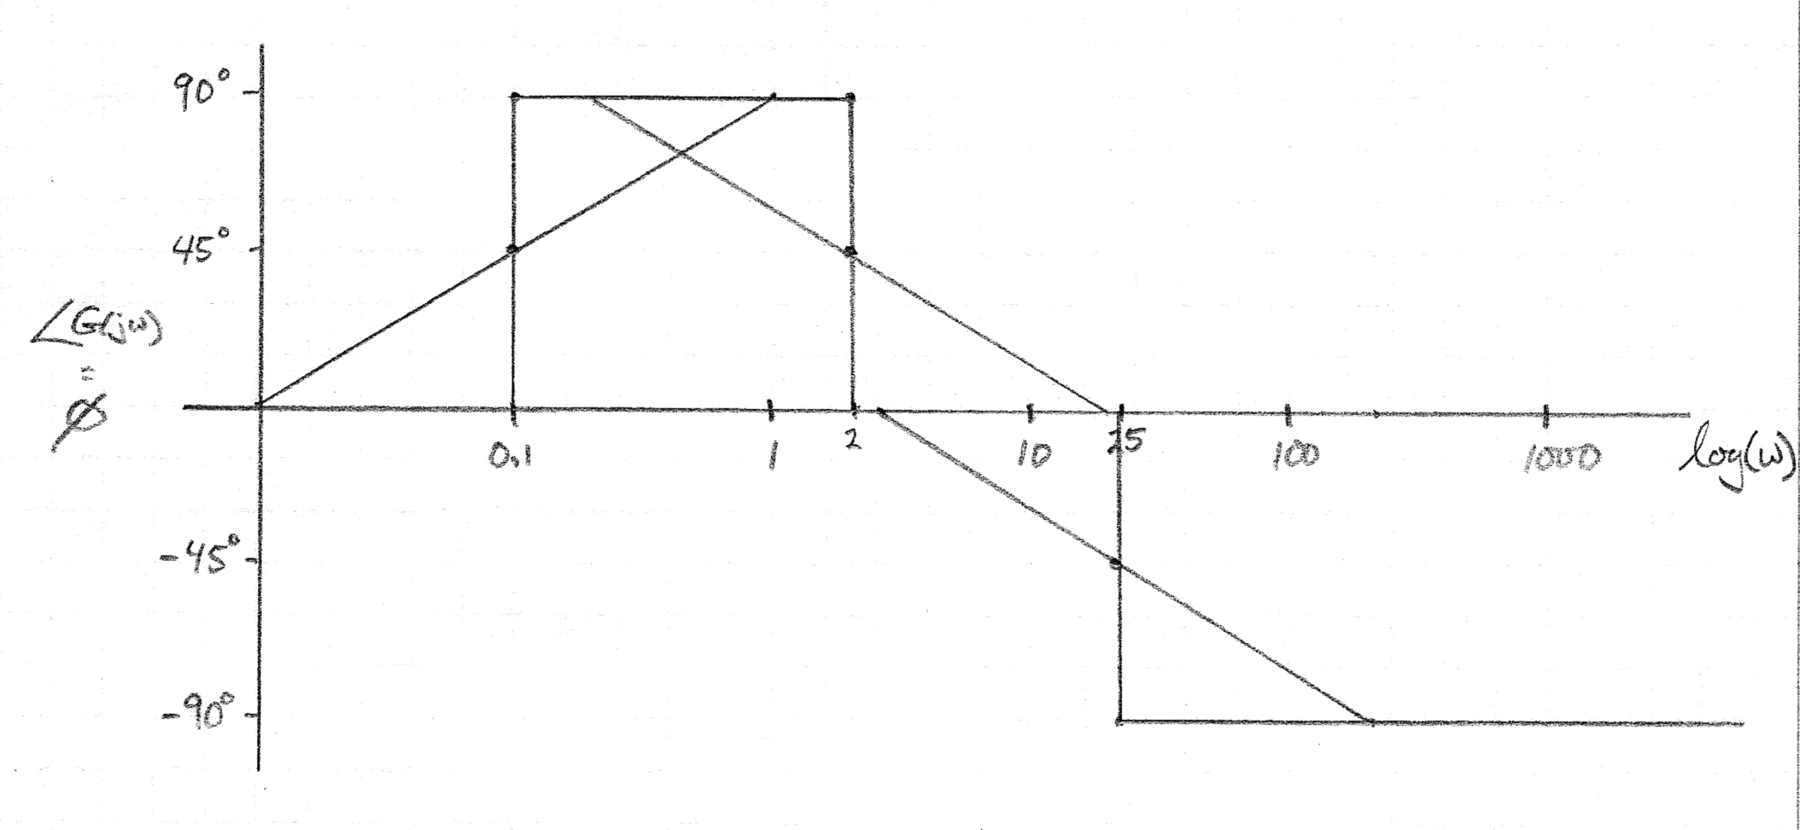
\includegraphics[width=5.5in]{figs05/00759a.png}

and finally, using a bit of artistic license, the smooth curves can be drawn in:

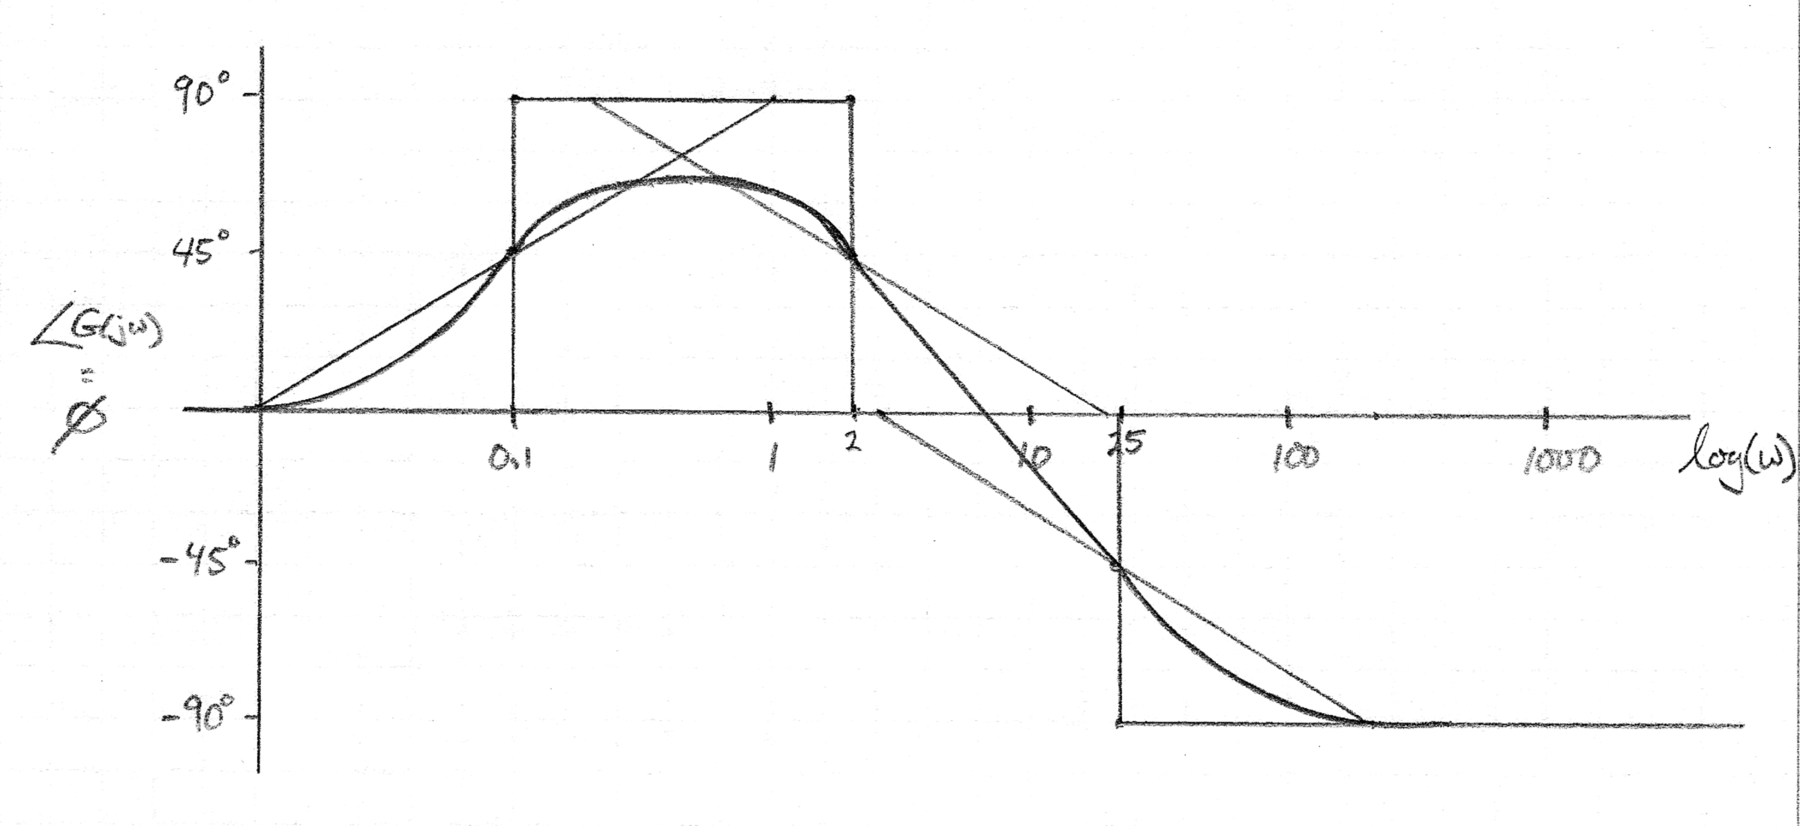
\includegraphics[width=5.5in]{figs05/00760a.png}


\end{Example}


\subsection{Poles or zeros at the origin}

It is slightly trickier to draw the Bode plots when there are one or more poles at $s=0$ because the first asymptotic approximation $\omega << a$ does not
apply.  In this case, there is a multiplicative term $1/s^n$, where $n$ is negative for poles at $s=0$ and positive for zeros at $s=0$.
For each value of $n$, the slope changes.  However, in all cases
\[
|s^n| = 1 \quad \mathrm{for} \;\omega=1 \quad\mathrm{and}\quad |s^n| = \omega^n
\]

Figure \ref{bodepolesatorigin} (Left) shows several Bode Magnitude plots of $s^n$.  Each plot is a straight line passing through the point, $\{0dB, \omega=1\}$.

\begin{figure}\centering
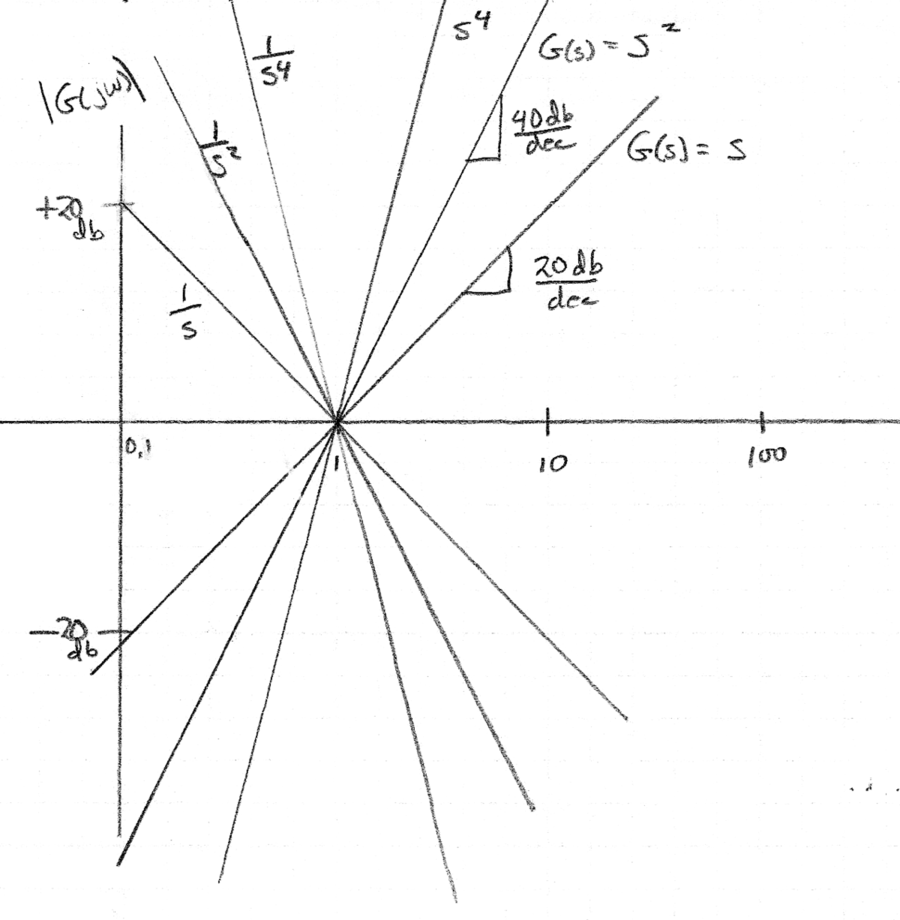
\includegraphics[width=3.0in]{figs05/00761a.png}
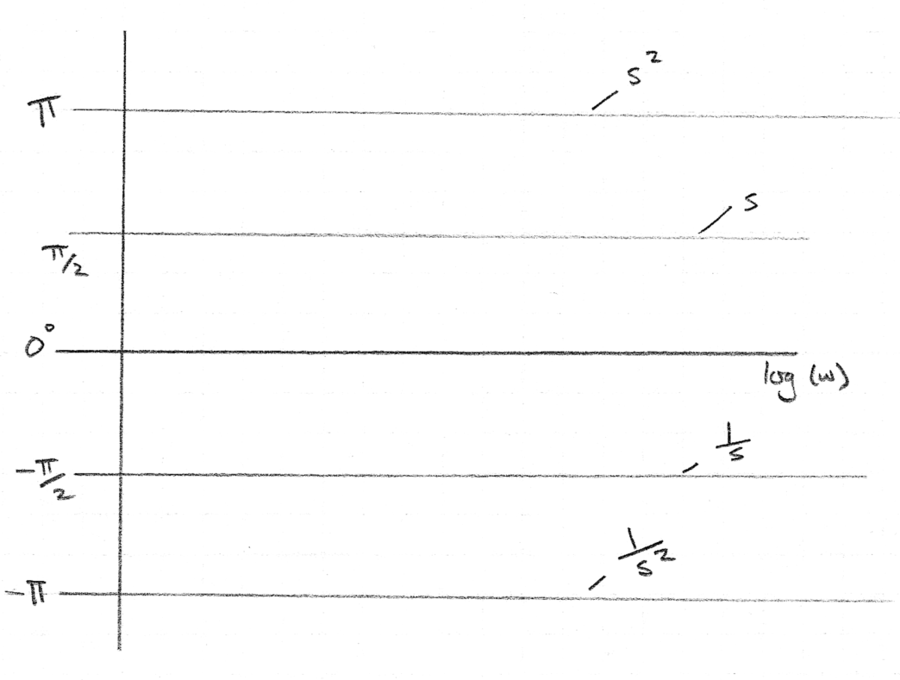
\includegraphics[width=3.0in]{figs05/00762a.png}
\caption{Bode Magnitude and Phase Plots of $G(s) = s^n$.  Left: The magnitude plots all pass through the point $\{1,0\}$. Right: Each term of $s^n$ contributes $n\times90^\circ$.}\label{bodepolesatorigin}
\end{figure}
%
% When a transfer function containing various poles and zeros also has poles or zeros at $s=0$, sketching the Bode Asympototic Magnitude Plot is slightly different because it does not begin with a horizontal asymptote at small values of $\omega$ ($\omega << \min(p_i, z_i)$).

For transfer functions containing poles or zeros at the origin, we need to choose a specific frequency (often $\omega=1$) at which to evaluate the magnitude of the transfer function.   We also compute the slope of the low-frequency asymptote at $\omega \approx 0$ by looking at the exponent of the pole or zero as $\omega\to 0$.  The phase contribution of poles or zeros at the origin (Figure \ref{bodepolesatorigin}, Right) is easier because it is just a constant $90^\circ$ for each power of $s$ in the numerator and $-90^\circ$ for each power of $s$ in the denominator.


\begin{Example}
Sketch the BAMP of the following transfer function
\[
G(s) = \frac      {(s+0.31)}       {s(s+10^{-2})(s+500)}
\]

First, we note that there is a single pole at $s=0$.    In order to find the vertical range of the plot, we need to compute the magnitude at some frequency below the non-zero poles and zeros.   Since the smallest feature is $s=0.01$, we choose $\omega=10^{-3}$.  Computing the magnitude  (to one or two significant figures)
\[
|G(j0.001)| \approx  \frac   {0.31}    {10^{-3}\times1.1\times10^{-2}\times500}
\]
\[
|G(j0.001)| \approx  {-10dB} + 60dB + 39dB - 54dB = 35dB
\]

The slope at this frequency is going to be $-20dB/$decade (Figure \ref{bodepolesatorigin}, Left) because the non-zero poles and zero do not contribute to the slope at $\omega = 10^{-3}$.    The magnitude will go down from there and the slope will change as the poles and zero become ``active''.   Plotting from the point $\{0.001, 35dB\}$ with slope -20$dB$/dec, and continuing with increasing $\omega$ we get

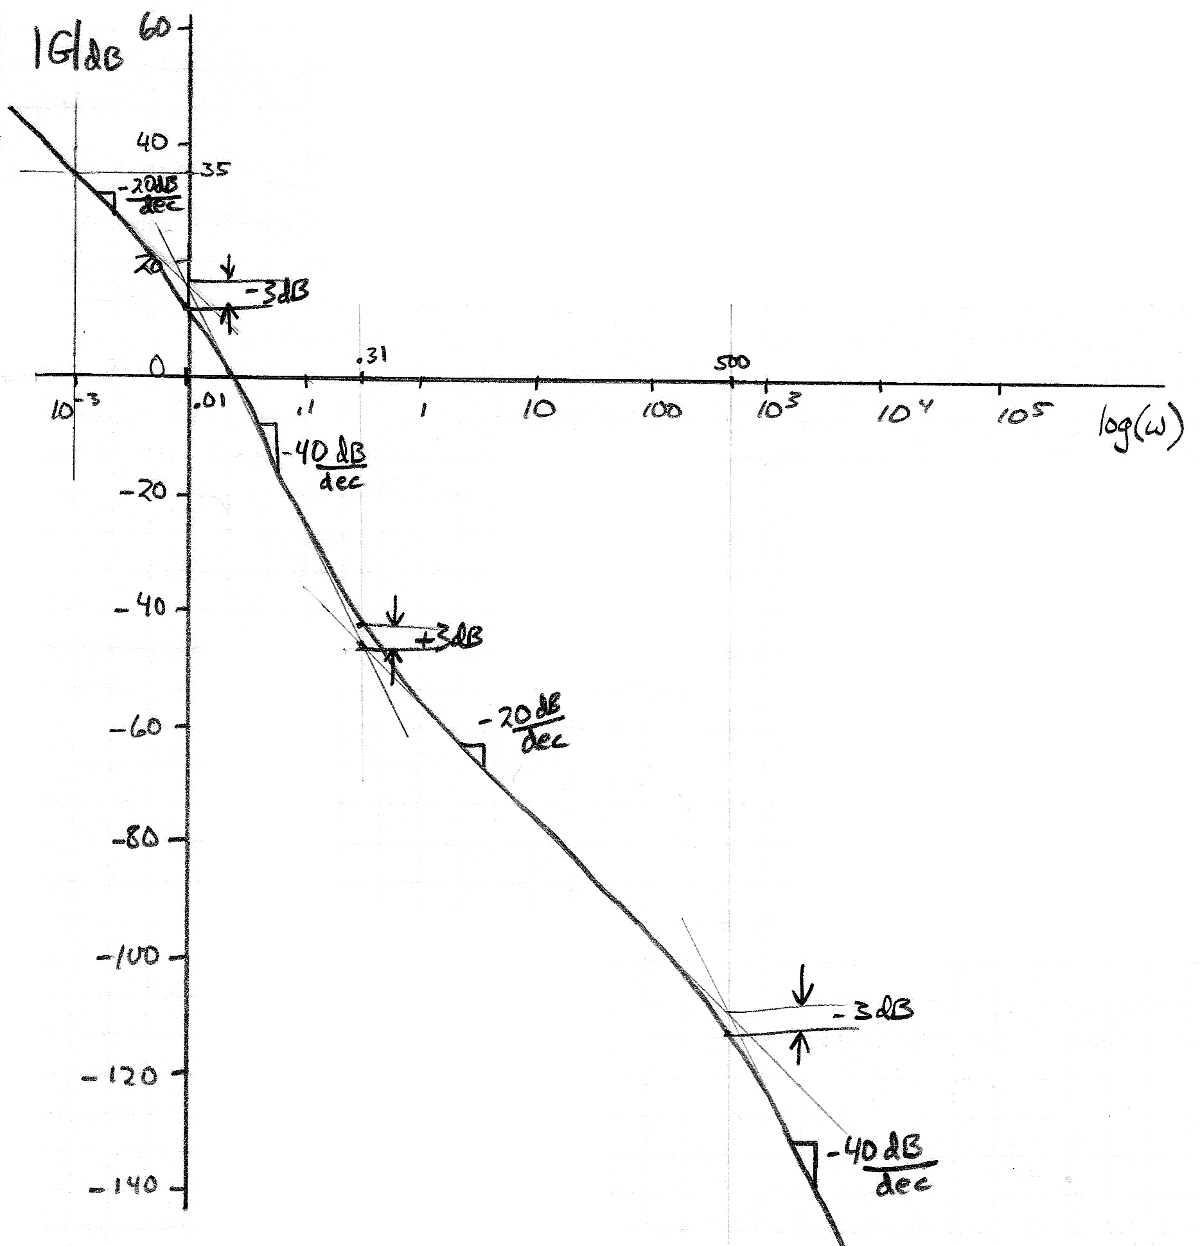
\includegraphics[width=5.0in]{figs05/00966.png}

Since this transfer function has 3 poles and only one zero, it's magnitude drops sharply with frequency.

\end{Example}


\subsection{Complex Conjugate Poles}

The BAMPs above were restricted to real-valued poles and zeros.  In this section we consider the BAMP of transfer functions having at least one pair of complex conjugate poles:

\[
p_i = a \pm jb
\]

As before, we are only interested in the case where $a<0$ so that the response is stable (does not grow with time).  A more typical system has a mixture of real and complex poles and zeros such as
\[
G(s) =  \frac {(s+5)} {(s+0.1)(s+1+3j)(s+1-3j)}
\]
we will see that it is more convenient to do the BAMP as well as the phase plot when the complex conjugate poles are represented in polar form, that is in terms of $\omega_n$ and $\zeta$.  Multiplying the complex poles,
$(s+1+3j)$ and $(s+1-3j)$ together,
\[
G(s) = \frac  {(s+5)}  {(s+0.1) (s^2 + 2s + 10 )  }
\]

Using the standard polar form for the second order term in the demoninator we have

\[
G(s) = \frac  {(s+5)}  {(s+0.1) (s^2 + 2\zeta\omega_n s + \omega_n^2)}
\]

where $\omega_n = \sqrt{10} = 3.1$ and $2\zeta\omega_n = 2 \to \zeta = 1/\omega_n = \frac{1}{\sqrt{10}} $.

Let's focus in on the second order poles:
\[
P_2(s) =   \frac {1}{s^2 + 2\zeta\omega_n s + \omega_n^2 }
\]
The key idea is to analyze the asymptotes of the 2nd order poles, $P_2(s)$, as we did above,  considering three
cases for the value of $\omega$:

\begin{enumerate}
  \item $\omega << \omega_n$
  \item $\omega =  \omega_n$
  \item $\omega >> \omega_n$
\end{enumerate}

plugging in $s=j\omega$  we derive the magnitude for each case:

\begin{enumerate}
  \item $|P_2(j\omega)| \approx \frac {1}{\omega_n^2}$ (remember $0< \zeta < 1$)


  \item $|P_2(j\omega_n)| = \frac  {1}{|j^2\omega_n^2 + 2\zeta j \omega_n^2 + \omega_n^2|}  =
                               \frac{1}{|-\omega_n^2 + 2\zeta j \omega_n^2 + \omega_n^2|} =
                               \frac{1}{2\zeta \omega_n^2}$

  \item $|P_2(j\omega)| \approx \frac {1}{\omega^2}$
\end{enumerate}

For case 1 ($\omega << \omega_n$),

\[
dB(|\frac{1}{\omega_n^2}|) = -2dB(\omega_n) \quad \mathrm{(a\quad constant)}
\]

For case 2 ($\omega =  \omega_n$),

\[
|P_2(j\omega_n)| =  \frac {1}  {2\zeta \omega_n^2} \qquad \mathrm{(also\quad a\quad constant)}
\]
For now, lets assume $\zeta=1$ giving
\[
|P_2(j\omega_n)| =  \frac {1}  {2\omega_n^2}
\]

in $dB$
\[
dB(| \frac {1}  {2 \omega_n^2} |) =  -dB(2) -dB(\zeta) -2dB(\omega_n) = -2dB(\omega_n)-6dB
\]

For case 3 ($\omega >>  \omega_n$),

\[
dB(|1/\omega^2|) = -2dB(\omega) \to \frac {-40dB}  {decade}
\]

Case 1 and case 3 correspond exactly to the system
\[
G(s) = \frac {1}{(s+\omega_n)(s+\omega_n)}
\]


The $\omega >> \omega_n$ asympotote (3) slopes down at a -2 (-40$dB$/dec) slope.


For case 2, The key is to realize that $0<\zeta<1$ and therefore $-dB(\zeta) > 0$.
Consider case (2) for different values of $\zeta$.  For $\zeta = 1$, ($db(\zeta)=0$),

\[
dB(|P_2(j\omega_n)|) =  -dB(2) -dB(\zeta) -dB(\omega_n^2) = -6dB -2 dB(\omega_n)
\]
This is exactly like two real poles:
\[
P_2(s) = \frac {1}{(s+\omega_n)(s+\omega_n)}
\]

but now consider for $\zeta= 0.001$

\[
dB(|P_2(j\omega_n)|) =  -dB(2) -dB(\zeta) -dB(\omega_n^2) = -6dB -(-60)db -2 dB(\omega_n) = 54db-2dB(\omega_n)
\]

The magnitude is increased by $54dB$.   Thus, while the complex conjugate pole pair has two asymptotes which act just like two real poles at $\omega_n$, the behavior at $\omega \approx \omega_n$ depends on $\zeta$.
Specifically, we can go back to the Case 2 result:

\[
|P_2(j\omega_n)| =  \frac {1}  {2\zeta \omega_n^2}
\]
using $dB$ and the log properties:
\[
|P_2(j\omega_n)| = 0dB - dB(2) - dB(\zeta) - dB(\omega_n^2)
\]
Notice that for $\omega<<\omega_n$, the horizontal asymptote is at $- dB(\omega_n^2)$.  Thus at
$\omega=\omega_n$, we correct the amplitude with a peak or smooth portion based on $\zeta$ according
to
\[
\mathrm{Correction}\; = -6 -dB(\zeta) = -dB(2\zeta)
\]
(quite simple and this is an exact result, not an approximation!)

\begin{ExampleSmall}

Use the computer to plot the BAMP of
\[
G(s) =  \frac{8.7\times10^4(s+0.1)}    {(s+1.0)(s^2 + 2\zeta100s + 10^4)}
\]
For $\zeta = \{0.05, 0.1, 0.25, 0.5, 0.75, 0.99\}$.  Make all the plots superimposed on the same axes.


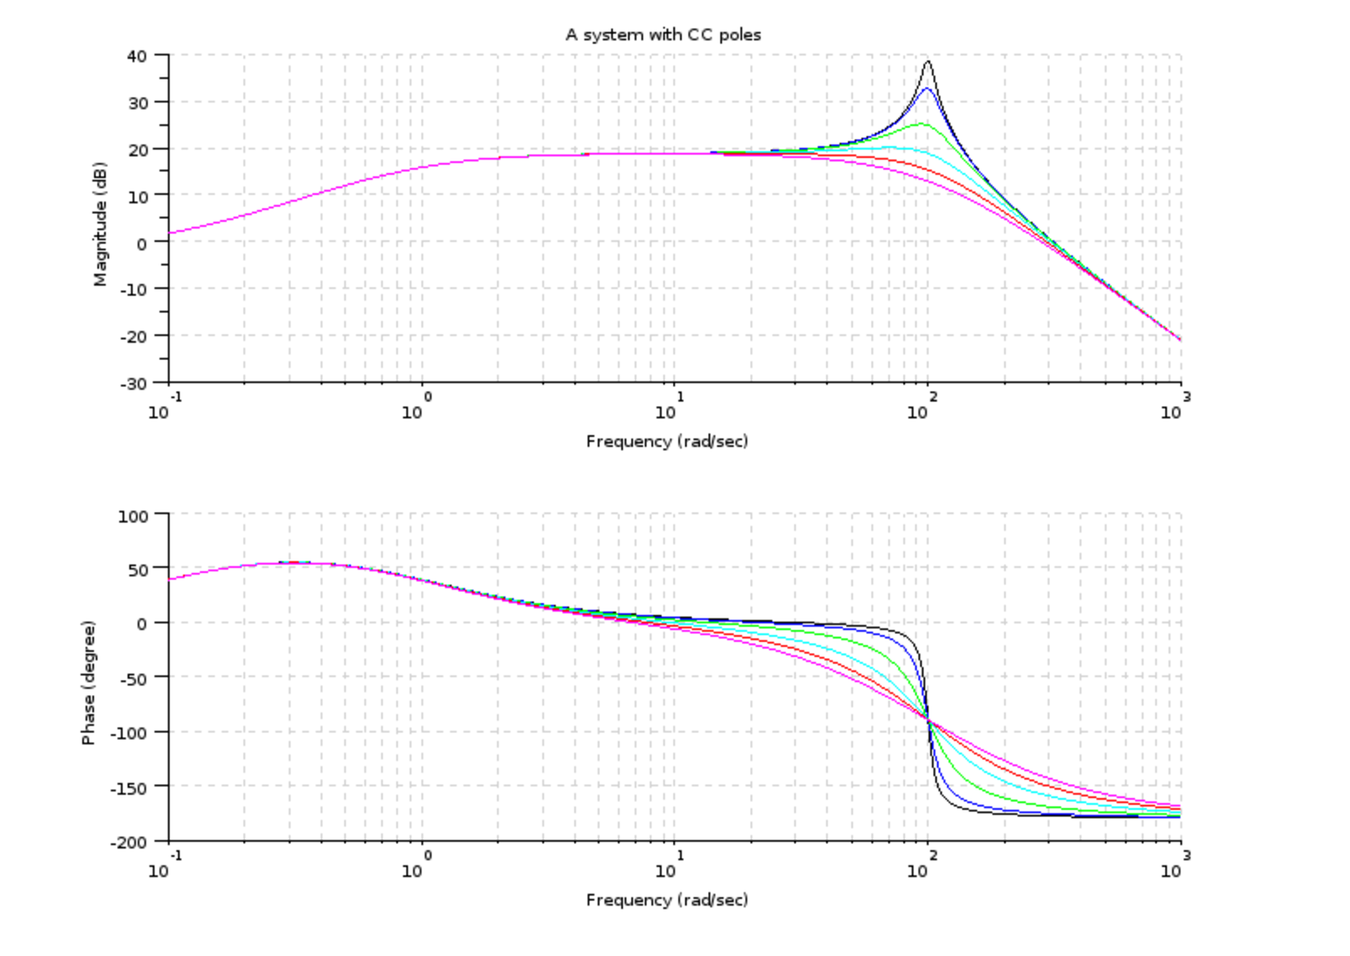
\includegraphics[width=4.5in]{figs05/zetasbodea.png}

\end{ExampleSmall}

\begin{ExampleCont}
Observations:

\begin{enumerate}
  \item As $\zeta$ approaches zero (dark blue), the magnitude plot has a sharper and sharper peak near $\omega=\omega_n$.
  \item As $\zeta$ approaches 1.0 (magenta), the magnitude plot smoothly curves through the point 6$dB$ below the intersection of the two straight line asymptotes.
  \item The high frequency asymptote has a slope of $-40dB/$decade.
  \item The Phase plot goes from $0^\circ$ to $-90^\circ$ as $\omega$ increases beyond $\omega_n$.

  \item As $\zeta$ approaches zero, the phase plot has a sharper transition $0^\circ \to -90^\circ$.
  \item As $\zeta$ approaches 1.0,  the phase plot acts like two real poles at $\omega = \omega_n$.
  \item When plotting the magnitude peak by hand,   make the peak hight
  \[
  -dB(2\zeta)
  \]
  above or below the horizontal asymptote.   Or roughly memorize this table:
\begin{center}
\begin{tabular}{c|r}
$\zeta$  & Peak (dB) \\\hline
0.001    &  $+54dB$ \\
0.05     &  $+20dB$ \\
0.1      &  $+12dB$  \\
0.25     &  $+6dB $  \\
0.5      &  $0dB$  \\
1.0      &  $-6dB $ \\
\end{tabular}\end{center}

  \item  Notice also in the computer output that the location  of the peak on the log $\omega$ axis
  shifts a bit lower than $\omega_n$ when $\zeta \to 1$.

\end{enumerate}

\end{ExampleCont}

\subsection{Complex Conjugate Zeros}


A system can also have complex conjugate zeros.  For example
\[
G(s) = \frac  {s^2 + 40s + 40,000}   {(s+0.1)(s+1000)^2}
\]
This system with three poles and two zeros has complex conjugate zeros at
\[
z_1 = -20+j199 \quad z_2 = -20-j199
\]


Zeros can also be expressed in terms of $\omega_n$ and $\zeta$ which in this case are
\[
\omega_n = |z_i| = \sqrt{-20^2 + 199^2} = 200.0 \qquad \zeta = -Re(z_i)/ \omega_n = -(-20)/200 = -0.1
\]

The frequency response of a complex conjugate pair of zeros is the inverse of a complex conjugate pair of poles.   Instead of a peak, there is a dip in the magnitude response and instead of a phase change of $-180^\circ$, there is a phase change of $+180^\circ$.

\begin{ExampleSmall}
Use the computer to plot the BAMP of
\[
G(s) =  \frac   {(s^2 + 2\zeta100s + 10^4)}   {(s+10)(s+30)(s+500)}
\]
For $\zeta = \{0.05, 0.1, 0.25, 0.5, 0.75, 0.99\}$.   Choose a frequency range which shows all the features of $G(s)$ (all the poles and zeros).   Make all the plots superimposed on the same axes.


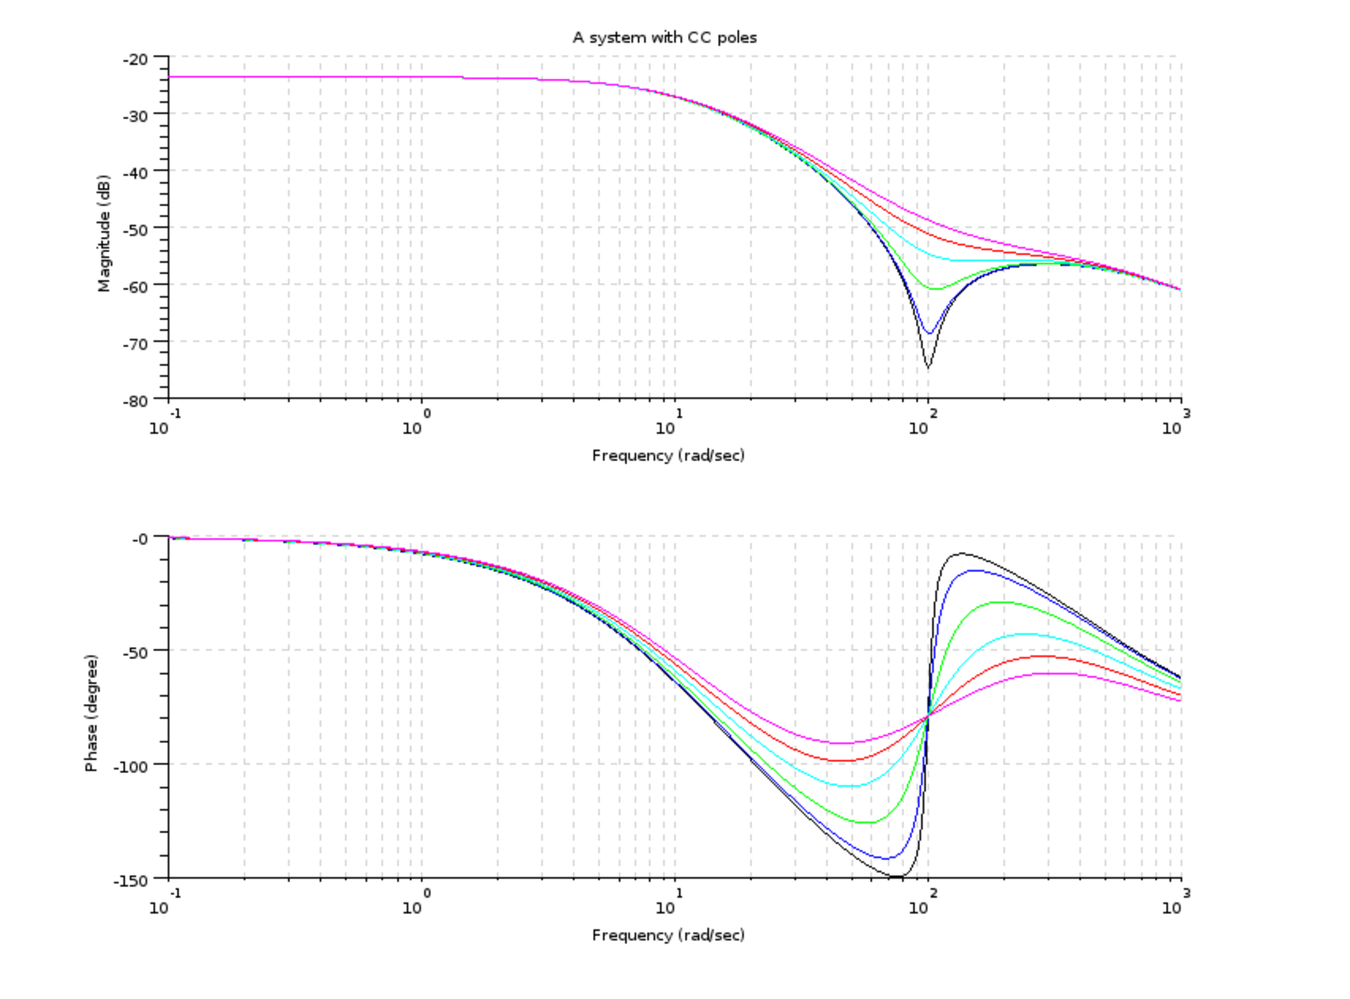
\includegraphics[width=4.5in]{figs05/zzetasbodea.png}

\end{ExampleSmall}




























% \section{Summary of Notation}

